\documentclass{article}
\usepackage{amsmath}
\usepackage{amssymb}

\title{房地产行业的数学模型}
\author{}
\date{}

\begin{document}

\maketitle

\begin{abstract}
中国房地产业在国民经济中起着举足轻重的作用。本文从定量的角度来实际分析房地产行业,建立一系列的数学模型,在模型的基础上综合分析,给对房价调控提供一些可行的建议。

基于联立方程组的住房的供给和需求模型。首先选取合理指标,通过非参数 Spearman 筛选指标,用 X12 方法进行季节调整。通过联立方程组建立需求和供给模型,然后使用高斯迭代方法进行验证,最后使用蛛网模型对围绕住房供给和需求模型进行分析。

基于 VAR 模型的房地产行业和国民经济其他行业关系模型。选取包括房地产行业在内的 14 个行业的投资额进行分析。首先通过 Spearman 参数检验,确定房地产和其他行业之间存在相关性。然后通过路径分析,确定各行业之间的直接和间接相关性。接着根据因果检验和协整检验,得到房地产行业与其他行业存在 granger 因果关系和长期协整关系。最后,为了进一步定量说明,采用向量自回归模型,建立房地产行业和国民经济其他 14 个主要行业的关系模型,并进行相应的脉冲分析和方差分解。

基于组合权重的 GC-TOPSIS 法的我国房地产行业态势分析模型,将房地产态势分为有效性因素和泡沫两大类进行讨论。对前几个模型进行分析,可知房地产的供需关系和房地产与其他行业的联系体现了其市场有效性。针对市场的泡沫,选取投资类,信贷类,居民承受能力等相关指标。通过客观熵值权重和主观的 AHP 权重相结合得到组合权重,然后使用 TOPSIS 法,得出理想方案和负理想方案,并对模型所需的评价方案进行标记。最后利用灰色关联给出房地产行业态势的评价模型。

基于离散 Hopfield 神经网络的房地产行业可持续发展模型。引入可持续发展指数,分为经济,社会,资源,调控管理四大块进行研究。首先基于态势分析模型可以得到我国房地产的经济发展情况。并选取人口密度等 6 个指标作为社会情况,选取人均公园绿地面积等 12 个指标作为资源情况,选取税率等 6 个指标作为调控管理情况。然后,利用离散 Hopfield 神经网络,对房地产可持续发展进行分级评判。最后,得到我国房地产行业可持续发展程度逐渐增高,可持续发展的等级越来越高。

基于博弈思想和 SVAR 的房价模型。首先,利用博弈思想,研究房地产业不同利益主体之间的博弈问题,得到价格形成的过程和研究房价模型的意义。然后,分别对经济适用房和商品房,选取可持续发展模型中经济,社会,资源,调控管理等因素及土地开发成本,建立关于房价的结构化向量自回归(SVAR)模型。最后,通过计算机仿真模拟房地产行业经济调控策略的成效,得到使房价下降 \(1\%\),\(2\%\),\(5\%\),\(10\%\) 时政府所应采取的措施。

最后,综合以上六个模型,对于我国房地产业,提出建议与意见。

关键词:联立方程组 VAR 离散 Hopfield 神经网络 GC-TOPSIS 博弈 SVAR
\end{abstract}

\section*{全国第八届研究生数学建模竞赛}

\section*{题目}

\textbf{房地产行业的数学模型}

\section*{目录}

\begin{itemize}
    \item 摘要 \dotfill 1
    \item 目录 \dotfill 3
    \item 1. 前言 \dotfill 5
        \begin{itemize}
            \item 1.1. 研究意义 \dotfill 5
            \item 1.2. 文献综述 \dotfill 5
            \item 1.3. 问题分析 \dotfill 6
            \item 1.4. 模型假设 \dotfill 6
            \item 1.5. 模型的符号和说明 \dotfill 6
            \item 1.6. 本文的架构设计 \dotfill 7
        \end{itemize}
    \item 2. 问题一、二解答——住房需求,供给模型 \dotfill 8
        \begin{itemize}
            \item 2.1. 指标的选取 \dotfill 8
            \item 2.2. 数据来源以及说明 \dotfill 10
            \item 2.3. 非参数 Spearman 秩和检验 \dotfill 12
                \begin{itemize}
                    \item 2.3.1. 斯皮尔曼等级相关系数的检验 \dotfill 12
                \end{itemize}
            \item 2.4. X12 方法季节调整 \dotfill 13
                \begin{itemize}
                    \item 2.4.1. X12 季节调整的理论 \dotfill 13
                    \item 2.4.2. X12 季节调整的结果 \dotfill 14
                \end{itemize}
            \item 2.5. 联立方程组模型 \dotfill 14
                \begin{itemize}
                    \item 2.5.1. 联立方程组的理论 \dotfill 14
                    \item 2.5.2. 供给需求联立方程求解 \dotfill 14
                \end{itemize}
            \item 2.6. 高斯迭代验证 \dotfill 16
            \item 2.7. 蛛网模型 \dotfill 17
        \end{itemize}
    \item 3. 问题三——房地产行业与其他行业关系模型 \dotfill 18
        \begin{itemize}
            \item 3.1. Spearman 检验 \dotfill 18
            \item 3.2. 路径分析 \dotfill 18
            \item 3.3. 单位根检验 \dotfill 20
            \item 3.4. Granger 因果检验 \dotfill 20
            \item 3.5. 协整检验 \dotfill 21
            \item 3.6. 滞后阶数确定 \dotfill 22
            \item 3.7. 向量自回归模型 \dotfill 23
                \begin{itemize}
                    \item 3.7.1. 模型的介绍 \dotfill 23
                    \item 3.7.2. 模型的求解 \dotfill 23
                    \item 3.7.3. 模型的检验 \dotfill 24
                \end{itemize}
            \item 3.8. 脉冲分析 \dotfill 25
            \item 3.9. 方差分解 \dotfill 25
        \end{itemize}
    \item 4. 问题四——房地产行业态势分析模型 \dotfill 27
        \begin{itemize}
            \item 4.1. 指标的选取 \dotfill 27
            \item 4.2. 权重计算 \dotfill 27
            \item 4.3. 理想点法(Topsis 法) \dotfill 28
            \item 4.4. 灰色关联度 \dotfill 29
            \item 4.5. 评价模型 \dotfill 30
        \end{itemize}
    \item 5. 问题五解答——房地产行业可持续发展模型 \dotfill 31
        \begin{itemize}
            \item 5.1. 指标的选取 \dotfill 32
            \item 5.2. Hopfield 神经网络模型介绍 \dotfill 32
            \item 5.3. 模型的建立 \dotfill 34
            \item 5.4. 结果分析 \dotfill 34
        \end{itemize}
    \item 6. 问题六解答——房价模型 \dotfill 35
        \begin{itemize}
            \item 6.1. 利益主体之间的博弈研究 \dotfill 35
            \item 6.2. 房价模型 \dotfill 37
                \begin{itemize}
                    \item 6.2.1. 经济适用房 \dotfill 37
                    \item 6.2.2. 商品房 \dotfill 40
                \end{itemize}
            \item 6.3. 政策模拟仿真 \dotfill 41
        \end{itemize}
    \item 7. 对我国房地产的建议和意见 \dotfill 42
    \item 8. 模型评价和推广 \dotfill 42
        \begin{itemize}
            \item 8.1. 模型的优点 \dotfill 42
            \item 8.2. 模型的缺点 \dotfill 42
            \item 8.3. 模型的推广 \dotfill 43
        \end{itemize}
    \item 参考文献 \dotfill 43
    \item 附录 \dotfill 44
\end{itemize}

\section{1. 前言}

\subsection{1.1 研究意义}

中国房地产业在国民经济中起着举足轻重的作用,房地产市场的健康稳定不仅是一个行业的问题,高房价蕴含着巨大的金融和社会风险。关注房地产市场波动,重要的不是房价本身,而是房地产市场供需是否平衡,结构是否合理,行业是否稳定,可持续发展是否健康。社会经济的发展对于房地产稳定发展的要求很高,房地产市场是市场经济体系的重要组成部分,是房地产业健康发展的载体。房地产市场的调控既是宏观经济调控的主要对象,又是房地产自身健康发展的有理保障。提高对房地产市场调控的规律性认识,引导房地产健康有序发展是一个重要的课题。

\subsection{1.2 文献综述}

随着我国改革开放的深入,国内的房地产行业露出了他强势的一面,成为带动国内经济发展的支柱产业和动力。根据国家发改委提供的数据,自 2002 年以来,一线城市的房价开始暴涨,04 年上涨了 19.8\%,05 年上涨 15.2\%,07 年上涨 12.8\%,08 年上涨 10.8\%,房价的上涨和房地产市场的供给和需求不无关系,而房价又反过来影响市场的供给和需求。如此的一个不良的循环,说明中国的房地产市场的畸形和不健全。房地产市场中,房价都是其表面上的运行核心。在一个稳定发展的市场下面,市场价格就会处在一个均衡的水平。要想研究房价,就必须对房地产市场的供给和需求有充分的认识和研究,从供需角度去研究就显得尤为重要。

房地产是典型的资金密集型企业,具有投资大、风险高、供应链长、地域性强的特点。由于房地产是我国国民经济的主导型产业,在现代经济生活中有着举足轻重的作用,与国民经济有着息息相关的作用。在房地产行业中,影响房地产走势的因素有宏观经济政策、金融政策、土地政策、房地产政策以及政府和房地产开发企业之间的关系。

在房地产环境中,构成经济环境的关键要素包括 GDP 的变化发展趋势、利率水平、居民可支配收入水平、汇率等影响经济增长的大事件。

构成社会环境的要素包括人口规模、年龄结构、消费心态和需求、收入分布、人口流动性、风俗和价值观念等等。不同城市、不同地区的人们对于房价的认同和接受能力是不一样的。

房地产作为生活资料满足人们的生活、享受和发展的需求,因为其位置的固定性、使用的长期性,可以使多种因素共同作用在这个经济实体上。

才员(2007)通过房地产市场的波动对国民经济和金融系统的影响,判断中国目前房地产市场泡沫情况。郑子濮(2004)利用多元统计的方法对中国过去 10 年的房地产进行了量化分析,分析了 03-04 年的房地产市场并未如同媒体所说的进入“房地产的冬天”。张雪娇(2004)从全局角度出发对房地产市场进行全方位、多角度的评价,提出了房地产市场和谐度评价的基本理论。余建源(2006)从房地产市场调控理论、房地产价格波动的特殊性理论以及中央和地方政府的利益和事权关系理论角度出发,找出我国房地产市场的不足。

\subsection{1.3 问题分析}

从经济学的角度来看,房地产的供需是一个市场密不可分的两个方面,把他们单独来分析反而不利于看到模型的本质。故把房地产供给模型和需求模型放在一起考虑,反而使得模型明朗化。

房地产行业和其他行业的相关性分析中最显而易见也是最重要的指标就是投资额,这个指标直接反应了整个行业的规模大小,具有很强的说服力。自向量回归采用的是一种非结构的方法来建立投资额这些内生变量的相关关系,为经济计量提供一种叫严密的说明,03年1月到11年8月的关于行业投资额的时间序列组成“向量”回归模型。

从积极性和泡沫性警告两个方面对房地产态势做出评价,做出两种因素的组合权重,利用理想点法 Topsis 求出灰色关联度,做出房地产态势的评价值。

模型一、二、三都是经济方面的模型,它们不能够完全反应房地产发展的整个态势,我们还需要从社会、资源以及政策的调控因素来评估房地产发展的态势和未来的走向。利用离散 Hopfield 神经网络引入可持续发展指数,分为经济、社会、资源、调控管理四大块合计24个衡量标准,对房地产可持续发展进行分级评判。其中经济指标来自于前几问的经济分析模型。

借助前几问已经得出的模型成果,加入房地产开发成本利用向量自回归做出全国性的总的一个房价模型。用计算机模拟仿真模拟房地产行业经济调控策略的成效。

\subsection{1.4 模型假设}

本文的基本假设如下:

(1) 假设在 2003 年至 2011 上半年之间,附件所有提供的数据正式可靠。

(2) 假设在 2003 年至 2011 上半年之间,无新的重大社会经济动荡和战争发生。

(3) 假设在 2003 年至 2011 上半年之间,我国各项宏观经济政策能及时准确地落实。

(4) 假设在 2003 年至 2011 上半年之间,我国对外经济政治政策无重大调整。

(5) 假设在 2003 年至 2011 上半年之间,我国对资本帐户管理政策无重大调整。

(6) 假设在 2003 年至 2011 上半年之间,无恶意国际炒家或机构扰乱金融市场。

(7) 假设在 2003 年至 2011 上半年之间,我国能对国际环境变化作出及时准确的反应。

(8) 假设所有人为理性人。

\subsection{1.5 模型的符号和说明}

\begin{table}
\centering
\begin{tabular}{c c c c c}
 & 商品房本 & 房地产 & 商品房销售 & 货币和准货 \\
 & 年竣工面 & 销售价 & 面积 & 币(M2)月末 \\
 & 积(万平方米) & 格指数 & (万平方米) & 数亿元) \\
1998-01 & 336 & 104.92 & 336 & 92211.4 \\
1998-02 & 327 & 104.12 & 378 & 92024 \\
1998-03 & 387 & 104.12 & 394 & 92015 \\
1998-04 & 441.14 & 104.62 & 490.46 & 92662 \\
1998-05 & 533.86 & 105.19 & 553.54 & 93936 \\
\end{tabular}
\caption{住房供给模型与各影响因素一览表(二)}
\end{table}

\begin{tabular}{c c c c c}
1998-06 & 811 & 105.42 & 814 & 94658 \\
1998-07 & 868.58 & 105.07 & 680.68 & 96314 \\
$\cdots$ & $\cdots$ & $\cdots$ & $\cdots$ & $\cdots$ \\
2010-10 & 5091.42 & 104.55 & 699776.74 & 9278.32 \\
2010-11 & 6531.01 & 104.34 & 710339.03 & 10112.72 \\
2010-12 & 27463.58 & 104.54 & 725851.79 & 21807.84 \\
\end{tabular}

\subsection{1.6 本文的架构设计}

本文不仅注重模型的建立还探讨了模型之间的内部联系和相互影响,从第四个模型开始,明显的用到了前面所得出的结论。

第一部分:前言,主要讲述了模型选取要求的背景,意义,以及当前的一些研究现状。

第二部分:将住房供给和需求模型联立成方程组,对影响因子进行 Spearman 检验,使用 X12 方法进行季节调整,联立方程得出结果,使用高斯迭代验证拟合度,最后使用蛛网模型进行一些拓展分析。

第三部分:主要是采用自回归向量模型来就房地产行业和其他的相关性行业做定量分析,在路径分析合理的大前提假设下,模型通过单位根检验,因果检验,协整检验,确定了滞后阶数,得出了向量自回归模型。

第四部分:从积极性和泡沫性警告两个方面对房地产态势做出评价,做出两种因素的组合权重,利用理想点法 Topsis 求出灰色关联度,做出房地产态势的评价值。

第五部分:利用离散 Hopfield 神经网络引入可持续发展指数,分为经济,社会,资源,调控管理四大块合计 24 个衡量标准,对房地产可持续发展进行分级评判。其中经济指标来自于前几问的经济分析模型。

第六部分:借助第五问的四个因素,加入房地产开发成本利用向量自回归做出全国性的总的一个房价模型。用计算机模拟仿真模拟房地产行业经济调控策略的成效。

整篇论文的结构如下所示:

\begin{figure}[h]
\centering
\includegraphics[width=\textwidth]{image.png}
\caption{论文结构图}
\end{figure}

\section{2. 问题一、二解答——住房需求,供给模型}

\subsection{2.1 指标的选取}

需求和供给是房地产销售的两只看不见的手决定着房地产的走势。这两个方面放在一起考虑。更加有利于对于房地产更加全面的认识。

对于住房需求我们选取了以下一些指标:

\begin{figure}[h]
\centering
\includegraphics[width=0.8\textwidth]{image1.png}
\caption{住房需求以及相关因素示意图}
\end{figure}

对于住房供给我们选择了另外一些具有说服力的指标。

\begin{figure}[h]
\centering
\includegraphics[width=0.8\textwidth]{image2.png}
\caption{住房供给以及相关因素示意图}
\end{figure}

根据经济学理论,选取了房地产销售价格指数,城镇家庭人均可支配收入,人均国民生产总值指数,储蓄存款,城镇人均建筑面积,年底城镇人口指数,结婚对数,房地产开发投资指数,房地产开发综合景气指数,房地产土地开发面积指数,房地产销售价格指数,货币和准货币(M2)。

\subsubsection{1. 房地产销售价格指数}

房屋销售价格指数是反映一定时期房屋销售价格变动程度和趋势的相对数,它是通过百分数的形式来反映房价在不同时期的涨跌幅度。包括商品房、公有房屋和私有房屋各大类房屋的销售价格的变动情况。

房屋销售价格指数的优点是“同质可比”,这种方法反映的是排除房屋质量、

建筑结构、地理位置、销售结构因素影响之后,由于供求关系及成本波动等因素带来的价格变动。

\subsubsection{2. 城镇家庭人均可支配收入}

指城镇居民家庭人均可用于最终消费支出和其它非义务性支出以及储蓄的总和,即居民家庭可以用来自由支配的收入。它是家庭总收入扣除交纳的所得税、个人交纳的社会保障费以及调查户的记账补贴后的收入。

\subsubsection{3. 人均国民生产总值指数}

人均国民生产总值(Per Capita Gross National Product 简写为 Per Capita G·N·P)指一国在一定时期内(通常为一年)生产的按市场价格计算的商品和劳务总值的按人口平均值。

一个国家的国民生产总值(GNP)除以该国国民人口的总数所得出的商。即指分摊到每个国民份上的国民生产总值的平均值。在经济学上,一般用来衡量或表示一个国家的经济发展程度。

\subsubsection{4. 储蓄存款}

城乡居民将暂时不用或结余的货币收入存入银行或其他金融机构的一种存款活动。又称储蓄。储蓄存款是信用机构的一项重要资金来源。

\subsubsection{5. 城镇人均建筑面积}

已经投入使用的居住总面积除以常住居民总人数,反映出一个城镇的大部分居民的生活水平。

\subsubsection{6. 年底城镇人口指数}

人口指数体现是是一个区域内的人口容量,间接的反馈出人口对于住房的需求。

\subsubsection{7. 结婚对数}

在当前社会形势下,有房已经成为了结婚一族的前提,中国 2010 年的结婚率是 $9\%_{0}$,新婚住房是一股强劲的购买力量。结婚率是指当年结婚对数占平均人口的比重。

\subsubsection{8. 房地产开发投资指数}

投资指数反应市场对于房地产市场的投资信心,如同股市是经济的晴雨表。直接影响商品房的完成情况。

\subsubsection{9. 房地产开发综合景气指数}

房地产景气指数,又称为景气度,指对企业景气调查中的定性经济指标通过定量方法加工汇总,综合反映某一特定调查群体或者发展趋势的一种指标。

\subsubsection{10. 房地产土地开发面积指数}

该指数反应了房地产板块的市场规模,以及可以提供的制定的区域做定性分析以及定量计算。

\subsubsection{11. 房地产销售价格指数}

房地产价格指数(Real estate price index)是反映房地产价格变动趋势和变动程度的相对数。它是通过百分数的形式来反映房价在不同时期的涨跌幅度。

\subsubsection{12. 货币和准货币(M2)}

准货币(quasi-money),又叫亚货币或近似货币,是一种以货币计值,虽不能直接用于流通但可以随时转换成通货的资产。准货币虽不是真正意义上的货币,但因可随时转化为现实的货币,故对货币流通有很大影响,是一种潜在货币。

准货币主要由银行定期存款、储蓄存款以及各种短期信用流通工具等构成, 10
如国库券储蓄存单、外汇券、侨汇券、金融卡等。
从货币层次上看,准货币=M2-M1。
准货币是潜在购买力,准货币=M2-M1,即广义货币与狭义货币之差成为准货币。具体包含一下几项:城乡居民储蓄存款、单位定期存款、证券公司保证金存款、其他存款。

\subsection{2.2 数据来源以及说明}
\begin{table}
\caption{住房需求模型与各影响因素一览表(一)}
\begin{tabular}{c c c c c c}
\hline
年份 & 商品房销售面积 & 城镇家庭人均可支配月收入 & 房地产销售价格指数 & 人均国内生产总值指数 & 储蓄存款(亿元) \\
 & (万平方米) & (元) & & & \\
\hline
1998-01 & 336 & 321.14 & 104.93 & 107.14 & 50119 \\
1998-02 & 378 & 334.95 & 104.13 & 107.05 & 50752 \\
1998-03 & 394 & 353.62 & 104.12 & 106.98 & 51374 \\
1998-04 & 490.46 & 359.33 & 104.62 & 106.91 & 51986 \\
1998-05 & 553.54 & 396.26 & 105.19 & 106.84 & 52587 \\
1998-06 & 814 & 408.52 & 105.42 & 106.78 & 53178 \\
1998-07 & 680.68 & 422.20 & 105.07 & 106.73 & 53759 \\
\ldots & \ldots & \ldots & \ldots & \ldots & \ldots \\
2010-10 & 9278.32 & 1520.97 & 104.55 & 110.40 & 338982 \\
2010-11 & 10112.72 & 1579.67 & 104.34 & 110.62 & 344979 \\
2010-12 & 21807.84 & 1674.98 & 104.54 & 110.85 & 351087 \\
\hline
\end{tabular}
\end{table}

注:当月商品房销售面积,当月城镇家庭人均收入可支配收入,房地产销售价格指数,储蓄存款的数据来源于题目所给的全国宏观月度库。

[TABLEENV:4]

[TABLEENV:5]

\begin{tabular}{l c c c}
\hline
 & R-squared & Adj.R-squared & Sum sq. resids \\
\hline
\(y\) & 0.966927 & 0.881182 & 0.638917 \\
\(x1\) & 0.964047 & 0.870837 & 2.160049 \\
\(x2\) & 0.932136 & 0.756192 & 0.880096 \\
\(x3\) & 0.970352 & 0.893487 & 0.709521 \\
\(x4\) & 0.952883 & 0.830729 & 1.676139 \\
\(x5\) & 0.966918 & 0.881148 & 0.723404 \\
\(x6\) & 0.953908 & 0.834411 & 3.169773 \\
\(x7\) & 0.960252 & 0.857203 & 1.926839 \\
\(x8\) & 0.959029 & 0.852807 & 3.296628 \\
\(x9\) & 0.943849 & 0.798272 & 1.722421 \\
\(x10\) & 0.926644 & 0.736462 & 3.062877 \\
\(x11\) & 0.958445 & 0.850710 & 1.401679 \\
\(x12\) & 0.922398 & 0.721209 & 5.321621 \\
\(x13\) & 0.958844 & 0.852143 & 1.309809 \\
\hline
\end{tabular}

\begin{tabular}{l c c c}
\hline
泡沫因素 & 熵值法权重 & 层次分析权重 & 组合权重 \\
\hline
房地产开发投资总额增速/ & & & \\
国内生产总值增速 & 0.054046 & 0.074074 & 0.015155 \\
房地产开发投资总额/ & & & \\
国内生产总值 & 0.144343 & 0.037037 & 0.020237 \\
房地产业投资总额增速/ & & & \\
固定资产投资完成额增速 & 0.896918 & 0.111111 & 0.377245 \\
房地产业投资总额/ & & & \\
固定资产投资完成额 & 0.052452 & 0.037037 & 0.007354 \\
房地产贷款/ & & & \\
总贷款 & 0.028181 & 0.148148 & 0.015804 \\
房地产贷款/ & & & \\
资金来源 & 0.067134 & 0.111111 & 0.028237 \\
空置率 & 0.1790693 & 0.1851852 & 0.1255279 \\
城市居民居住消费价格指数/ & & & \\
租房消费价格指数 & 0.25403801 & 0.1111111111 & 0.1068486 \\
房地产销售价格指数/ & & & \\
居民消费价格指数 & 0.522143 & 0.148148 & 0.292818 \\
房价收入比 & 0.076846 & 0.037037 & 0.010774 \\
\hline
\end{tabular}

\begin{tabular}{c c c c c}
1998-06 & 811 & 105.42 & 814 & 94658 \\
1998-07 & 868.58 & 105.07 & 680.68 & 96314 \\
$\cdots$ & $\cdots$ & $\cdots$ & $\cdots$ & $\cdots$ \\
2010-10 & 5091.42 & 104.55 & 699776.74 & 9278.32 \\
2010-11 & 6531.01 & 104.34 & 710339.03 & 10112.72 \\
2010-12 & 27463.58 & 104.54 & 725851.79 & 21807.84 \\
\end{tabular}

注:城镇居民人均建筑面积,年底城镇总人口数,商品房本年竣工面积(当月)来源于题目所给的全国宏观月度库,结婚对数来自中国统计年鉴。

\subsection{2.3 非参数 Spearman 秩和检验}

斯皮尔曼(Spearman)相关系数是描述两组变量之间是否存在着相同或相反趋同性的一种指标,由于该检验不需要假定服从正态分布,仅需要确定变量在每个点(时期)上的等级即可获得,因此具有较好的性质。在两组数据都没有重复观测值的情况下,斯皮尔曼等级相关系数的公式为:

\[
r_s = 1 - \frac{6 \sum d_i^2}{n(n^2 - 1)}
\]

其中 $d_i$ 表示两组数据之间的等级之差,n 为样本量。

Kendall 秩相关系数 $r_k$ 也可反映两组变量的等级或秩相关的程度。Kendall 秩相关系数 $r_k$ 又称为一致性系数或和谐系数。

设有两对观测值 $(x_{i_1}, y_{i_1})$ 与 $(x_{i_2}, y_{i_2})$,如果 $(x_{i_1}, y_{i_1})$ 的两个元素都比 $(x_{i_2}, y_{i_2})$ 的元素大,即 $x_{i_1} > x_{i_2}$ 且 $y_{i_1} > y_{i_2}$,则称 $(x_{i_1}, y_{i_1})$ 与 $(x_{i_2}, y_{i_2})$ 为和谐的,否则称它们为不和谐的。记 $N_c$ 为和谐观测值的对数,$N_d$ 为不和谐观测值的对数,如果没有相同的 $x_i$ 或相同的 $y_i$,则

\[
N_c + N_d = C_n^2 = \frac{n(n-1)}{2}, \quad r_k = \frac{2(N_c - N_d)}{n(n-1)}
\]

如果有相同的 $x_i$ 或相同的 $y_i$,则

\[
r_k = \frac{N_c - N_d}{N_c + N_d}
\]

这时,将所有 $x_{i_1} \neq x_{i_2}$ 的观测值对 $(x_{i_1}, y_{i_1})$ 与 $(x_{i_2}, y_{i_2})$ 进行比较。

当 $(x_{i_1} - x_{i_2})(y_{i_1} - y_{i_2}) > 0$ 时,给 $N_c$ 加 1;

当 $(x_{i_1} - x_{i_2})(y_{i_1} - y_{i_2}) < 0$ 时,给 $N_d$ 加 1;

当 $y_{i_1} = y_{i_2}$ 时,给 $N_c$ 与 $N_d$ 各加 0.5。

这样得到的 Kendall 秩相关系数 $r_k$ 又叫做 Gamma 系数,记作 $\gamma$。

\subsubsection{2.3.1 斯皮尔曼等级相关系数的检验}

和其它的推断一样,当以样本的数据来推测总体时,由于样本带有随机性,在小样本时数据间有相关,但总体之间不一定相关。因此有必要进行假设检验。在此,设定原假设 $H_0$:研究的总体之间无相关(即 $\rho = 0$),备择假设 $H_1$:研究的总体之间有相关(即 $\rho \neq 0$)。

检验的样本估计量为样本的相关系数 \( r_s \),在小样本的情况下通常临界值的 \( r \) 可直接查表,但大样本的情况下可以通过变换

\[
t = r_s \sqrt{\frac{n-2}{1-r_s^2}}
\]

服从 \( t_{(n-2)} \) 的 \( t \) 分布,运用 SAS 软件,进行 \( t \) 检验,得到住房需求与各指标的斯皮尔曼检验结果如表 6

\textbf{表6 住房需求模型斯皮尔曼检验结果}

\begin{table}
\caption{住房需求模型与各影响因素一览表(一)}
\begin{tabular}{c c c c c c}
\hline
年份 & 商品房销售面积 & 城镇家庭人均可支配月收入 & 房地产销售价格指数 & 人均国内生产总值指数 & 储蓄存款(亿元) \\
 & (万平方米) & (元) & & & \\
\hline
1998-01 & 336 & 321.14 & 104.93 & 107.14 & 50119 \\
1998-02 & 378 & 334.95 & 104.13 & 107.05 & 50752 \\
1998-03 & 394 & 353.62 & 104.12 & 106.98 & 51374 \\
1998-04 & 490.46 & 359.33 & 104.62 & 106.91 & 51986 \\
1998-05 & 553.54 & 396.26 & 105.19 & 106.84 & 52587 \\
1998-06 & 814 & 408.52 & 105.42 & 106.78 & 53178 \\
1998-07 & 680.68 & 422.20 & 105.07 & 106.73 & 53759 \\
\ldots & \ldots & \ldots & \ldots & \ldots & \ldots \\
2010-10 & 9278.32 & 1520.97 & 104.55 & 110.40 & 338982 \\
2010-11 & 10112.72 & 1579.67 & 104.34 & 110.62 & 344979 \\
2010-12 & 21807.84 & 1674.98 & 104.54 & 110.85 & 351087 \\
\hline
\end{tabular}
\end{table}

\textbf{表7 住房供给模型斯皮尔曼检验结果}

[TABLEENV:4]

\subsection{2.4 X12 方法季节调整}

\subsubsection{2.4.1 X12 季节调整的理论}

季节性变动的发生,不仅是由于气候的直接影响,而且社会制度及风俗习惯也会引起季节变动。经济统计中的月度和季度数据或大或小都含有季节变动因素,以月份或季度作为时间观测单位的经济时间序列通常具有一年一度的周期性变化,这种周期变化是由于季节因素的影响造成的,在经济分析中称为季节性波动。经济时间序列的季节性波动是非常显著的,它往往遮盖或混淆经济发展中其他客观变化规律,以致给经济增长速度和宏观经济形势的分析造成困难和麻烦。因此,在进行经济增长分析时,必须去掉季节波动的影响,将季节要素从原序列中剔除,这就是所谓的“季节调整” (Seasonal Adjustment)。

设 \( Y_t \) 表示一个无奇异值的月度时间序列,通过预测和回推来扩展序列使得在序列的尾端不需要对季节调整公式进行修改。把 \( Y_t \) 分解为趋势循环项

TCt、季节项 \( S_t \) 和不规则要素 \( I_t \)。我们这里采用对数加法实现季节调整:

对数加法模型:
\[
\ln Y_t = \ln TC_t + \ln S_t + \ln I_t
\]

\subsubsection{2.4.2 X12 季节调整的结果}

图 3 表示季节调整后需求量和供应量的实际值

\begin{figure}[h]
    \centering
    \includegraphics[width=0.8\textwidth]{image.png}
    \caption{季节调整后供给和需求示意图}
    \label{fig:seasonal_adjustment}
\end{figure}

\subsection{2.5 联立方程组模型}

\subsubsection{2.5.1 联立方程组的理论}

经济系统并没有严格的空间概念。国民经济是一个系统,一个地区的经济也是一个系统,甚至某一项经济活动也是一个系统。例如我们进行商品购买决策,由于存在收入或预算的制约,在决定是否购买某一种商品时,必须考虑到对其他商品的需求与其他商品的价格,这样,不同商品的需求量之间是互相影响、互为因果的。那么,商品购买决策就是一个经济系统。

联立方程系统就是一组包含未知数的方程组。利用一些多元方法可以对系统进行估计,这些方法考虑到了方程之间的相互依存关系。

\subsubsection{2.5.2 供给需求联立方程求解}

因为需求与住房供应有关,同时供应也与需求有关,故联立方程得到住房供需函数联立方程如下:
\begin{align*}
a_1(t) &= -29.694462911194 + 0.820086189462682 \, b_1(t) + 0.331286350625579 \, a_2(t) \\
&+ 0.611919650814839 \, a_3(t) + 7.28255203715754 \, a_4(t) + 0.691246556344289 \, a_5(t) \\
&+ 0.695101407992393 \, a_6(t) + 1.30775681762088 \, a_7(t) + 0.0480918132438054 \, a_8(t) \\
b_1(t) &= 0.289229749812516 + 0.539283785307939 \, a_1(t-1) - 3.0484445085418 \, b_2(t) \\
&+ 5.08529330158403 \, b_3(t) + 0.279524705819216 \, b_4(t) + 0.265380623606964 \, b_5(t) \\
&+ 1.77027412187801 \, a_3(t)
\end{align*}
其中 \( a_i = \log(x_i - sa) \quad i = 1, 2, \ldots, 8 \quad c_j \) 为相应的系数 \quad \( j = 1, \ldots, 16 \)

\begin{table}[h]
    \centering
    \caption{政策模拟仿真结果}
    \label{tab:35}
    \begin{tabular}{c c c c c}
        \hline
        & 房价下降比 & 上调1\% & 上调2\% & 上调5\% & 上调10\% \\
        \hline
        \( x_1 \) 房地产开发投资指数 & & 0.12\% & 0.25\% & 0.67\% & 1.43\% \\
        \hline
    \end{tabular}
\end{table}

\begin{tabular}{l c c c c}
x2税收政策干预指数 & 0.61\% & 1.32\% & 3.45\% & 6.08\% \\
x3房地产信贷监管指数 & 0.54\% & 1.20\% & 1.56\% & 4.56\% \\
x4房地产风险调控指数 & 0.44\% & 1.01\% & 1.34\% & 4.08\% \\
\end{tabular}

\begin{table}
\centering
\begin{tabular}{c c c c c}
\hline
b1 & b2 & b3 & b4 & b5 \\
\hline
商品房本年 & 房地产开发 & 房地产开发 & 房地产土地 & 货币和准货 \\
竣工面积 & 投资指数 & 综合景气指数 & 开发面积指数(直接影响供应量) & 币(M2) \\
万平方米 & & & & 亿元 \\
\hline
\end{tabular}
\end{table}

其中 $a_{i} = \log(x_{i} - sa), \, i = 1, 2, \dots, 8$

利用 Eviews 进行计算,得出的系数进行相应的参数以及拟合度检验,公式的拟合度如表10所示,说明说联立方程组和实际情况吻合度很高

\begin{table}
\centering
\begin{tabular}{c c}
\hline
拟合度 & \\
\hline
方程(1) & 0.984380 \\
方程(2) & 0.964041 \\
\hline
\end{tabular}
\caption{表10 方程的拟合度}
\end{table}

然后对两个方程进行必要的残差检验,住房需求公式的残差如图4所示,住房供给公式的残差如图5所示

\begin{figure}[h]
\centering
\includegraphics[width=0.8\textwidth]{A1_Residuals.png}
\caption{图5 住房需求模型残差检验}
\end{figure}

\begin{figure}[h]
    \centering
    \includegraphics[width=0.8\textwidth]{B1_Residuals.png}
    \caption{B1 Residuals}
    \label{fig:B1_Residuals}
\end{figure}

图6 住房供给模型残差检验

最后得出以下的住房需求模型:
\begin{align*}
a_1(t) &= -29.694462911194 + 0.820086189462682 \, b_1(t) + 0.331286350625579 \, a_2(t) \\
&+ 0.611919650814839 \, a_3(t) + 7.28255203715754 \, a_4(t) + 0.691246556344289 \, a_5(t) \\
&+ 0.695101407992393 \, a_6(t) + 1.30775681762088 \, a_7(t) + 0.0480918132438054 \, a_8(t) \\
b_1(t) &= 0.289229749812516 + 0.539283785307939 \, a_1(t-1) - 3.0484445085418 \, b_2(t) \\
&+ 5.08529330158403 \, b_3(t) + 0.279524705819216 \, b_4(t) + 0.265380623606964 \, b_5(t) \\
&+ 1.77027412187801 \, a_3(t)
\end{align*}
其中 $a_i = \log(x_i \_ sa) \quad i = 1, 2, 3$

\subsection{2.6 高斯迭代验证}

在得出具体的系数之后,我们通过高斯迭代法进行模拟检测,得出图6住房需求模型的实际值和拟合值的示意图,图7是住房供给模型的实际值和拟合值的示意图。

\begin{figure}[h]
    \centering
    \includegraphics[width=0.8\textwidth]{Housing_Demand_Model.png}
    \caption{住房需求模型}
    \label{fig:Housing_Demand_Model}
\end{figure}

其中,实际值为蓝线,而拟合值为红线。

\begin{figure}[h]
    \centering
    \includegraphics[width=0.8\textwidth]{image1.png}
    \caption{住房供给模型实际值和拟合值}
    \label{fig:8}
\end{figure}

其中,实际值为蓝线,而拟合值为红线。

从图可以看出,拟合值和实际值拟合的比较好,公式被采纳。

\subsection{2.7 蛛网模型}

经济学中的蛛网模型运用弹性原理解释某些生产周期较长的商品在失去均衡时发生的不同波动情况的一种动态分析理论。

\( x_{k} \) ~ 第k时段商品供给;\( y_{k} \) ~ 第k时段商品需求

\begin{equation}
y_t = (I_k - \Phi_1 L - \cdots - \Phi_p L)^{-1} \varepsilon_t = (I_k + A_1 L + A_2 L^2 + \cdots) \varepsilon_t \quad t = 1, 2, \ldots, T
\end{equation}

消费者对于需求的敏感程度 \quad 生产者对于供应的敏感程度

小,有利于经济稳定, \quad 小,有利于经济稳定 \quad 所以 \quad \( <1 \), 经济稳定

故而,需求函数 \( y_{k} = f(x_{k}) \),供应函数 \( y_{k} = g(x_{k+1}) \)。

\begin{figure}[h]
    \centering
    \includegraphics[width=0.8\textwidth]{image2.png}
    \caption{蛛网模型的验证效果}
    \label{fig:9}
\end{figure}

西方经济学家认为,蛛网模型解释了某些生产周期较长的商品的产量和价格的波动的情况,是一个有意义的动态分析模型。但是,这个模型还是一个很简单的和有缺陷的模型。这是因为,根据该模型分析,造成产量和价格波动的主要原因是:生产者总是根据上一期的价格来决定下一期的产量,这样,上一期的价格同时也就是生产者对下一期的预期价格。而事实上,在每一期,生产者只能按照本期的市场价格来出售由预期价格(即上一期价格)所决定的产量。这种实际价格和预期的价格不吻合,造成了产量和价格的波动。但是,这种解释是不全面的。因为生产者从自己的经验中,会逐步修正自己的预期价格,使预期价格接近实际价格,从而使实际产量接近市场的实际需求量。

蛛网模型的趋势结果表明,房地产目前正处于一个非均衡的阶段,每次调控措施的出台都会导致结果偏离平衡点更多。说明房地产商预定的房价与实际的不否,并且没有修正自己的价格。

\section{3. 问题三——房地产行业与其他行业关系模型}

从投资总额角度入手,把房地产开发与农林牧副渔业,通信设备、计算机以及其他电子设备制造业,纺织业,农副食品加工业,制造业,煤炭开采以及洗选业,采矿业,林业,建筑业,有色金属矿采选业,教育业,金融业,科学研究、技术服务和地址勘察业。图 9 是 2003 年 1 月和 2011 年 8 月每个行业各自所占的比例份额。

\begin{figure}[h]
\centering
\includegraphics[width=\textwidth]{image.png}
\caption{各行业所占投资比例}
\end{figure}

\subsection{3.1 Spearman 检验}

根据前面所叙述的方法,我们进行 Spearman 的非参数检验。最后结果可得各个行业投资均通过检验。

\subsection{3.2 路径分析}

路径分析模型是由美国遗传学家 Swell Wright 于 1921 年首创,用于研究多个变量之间多层因果关系及其相关强度的方法,现已发展成为社会学的主要研究方法之一。路径分析的主要目的是检验一个假想的因果模型的准确和可靠程度,测量变量间因果关系的强弱,回答下述问题:1. 模型中两变量 \(x_j\) 与 \(x_i\) 间是否存在相关关系;2. 若存在相关关系,则进一步研究两者间是否有因果关系;3. 若 \(x_j\) 影响 \(x_i\),那么 \(x_j\) 是直接影响 \(x_i\),还是,通过中介变量间接影响或两种情况。

况都有;4 直接影响与间接影响两者大小如何。

该模型实际上就是一特定的网络图形描述的标量之间的线性关系的假设, 模型的建立必须经过理论论证, 将总的效果分解成为直接效应、间接效应和联合效应, 然后将有关变量按照推理的层次和因果关系顺序排列, 然后按照结果模型画出路径图。

设有因变量 \( y \) 以及自变量 \( x_1 \) 与 \( x_2 \), 而 \( x_1 \) 与 \( x_2 \) 的关系不确定、其简单相关系数 \( r_{12} \neq 0 \)。

如果将 \( x_1 \) 与 \( x_2 \) 对 \( y \) 的影响图解为

\[
\begin{tikzpicture}[node distance=2cm, auto]
    \node (x1) {$x_1$};
    \node (x2) [below of=x1] {$x_2$};
    \node (y) [right of=x1, node distance=3cm] {$y$};
    
    \draw[->] (x1) -- node [left] {$r_{12}$} (x2);
    \draw[->] (x1) -- (y);
    \draw[->] (x2) -- (y);
\end{tikzpicture}
\]

则称 \( x_1 \) 或 \( x_2 \) 指向 \( y \) 的连接线 \( x_1 \to y \) 及 \( x_2 \to y \) 为直接通径, 称 \( x_1 \to x_2 \to y \) 及 \( x_2 \to x_1 \to y \) 为间接通径。

类似的, 如果有多个自变量 \( x_1, x_2, x_3, \ldots, x_m \) 存在, 则称 \( x_i \) 指向 \( y \) 的连接线 \( x_i \to y \) 为直接通径, 称 \( x_{j_1} \to x_{j_2} \to y \) 或者 \( x_{j_2} \to x_{j_1} \to y \) 为间接通径, 这里的 \( j, j_1, j_2 = 1, 2, \ldots, m \) 且 \( j_1 \neq j_2 \)。

在直接通径 \( x_j \to y \) 上, 若 \( x_j \) 的取值增加一个标准单位时, \( y \) 将要改变的标准差单位数 \( p_j \) 成为通径 \( x_j \to y \) 的系数。\( x_j \) 增加时, 若 \( y \) 也增加, 则 \( p_j > 0 \); \( x_j \) 增加时, 若 \( y \) 反而减少, 则 \( p_j < 0 \)。

因此, 通径系数 \( p_j \) 可以看作是 \( x_j \) 对 \( y \) 的标准效应, 而 \( p_j \) 的绝对值反映 \( x_j \) 对 \( y \) 的标准影响力。可以根据 \( p_j \) 的绝对值确定 \( x_j \) 对于改变 \( y \) 的取值的相对重要性。对行业投资额进行路径分析的结果如下:

\[
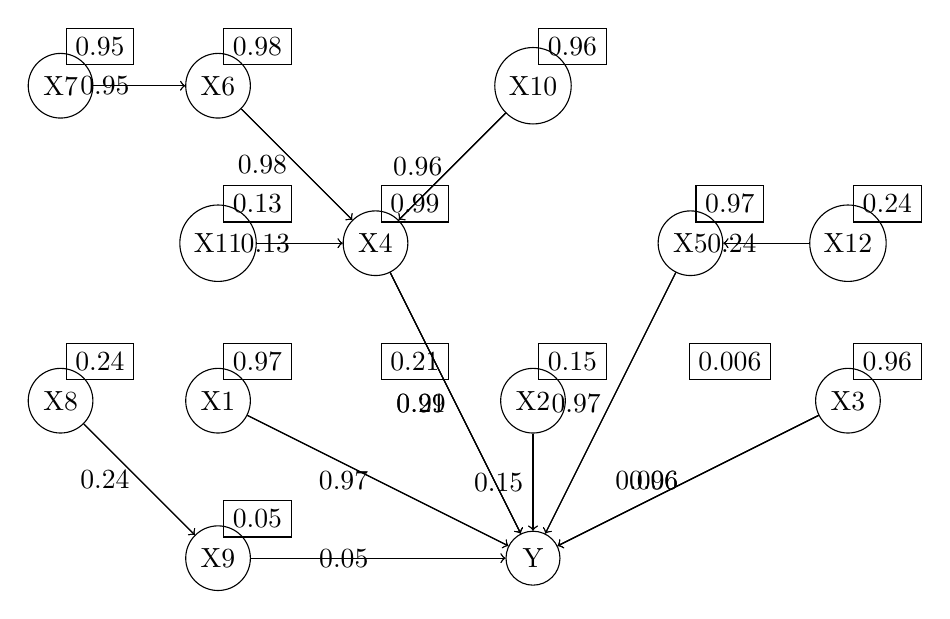
\begin{tikzpicture}[node distance=2cm, auto]
    % Define nodes
    \node (x1) at (0,0) [circle, draw] {X1};
    \node (x2) at (4,0) [circle, draw] {X2};
    \node (x3) at (8,0) [circle, draw] {X3};
    \node (x4) at (2,2) [circle, draw] {X4};
    \node (x5) at (6,2) [circle, draw] {X5};
    \node (x6) at (0,4) [circle, draw] {X6};
    \node (x7) at (-2,4) [circle, draw] {X7};
    \node (x8) at (-2,0) [circle, draw] {X8};
    \node (x9) at (0,-2) [circle, draw] {X9};
    \node (x10) at (4,4) [circle, draw] {X10};
    \node (x11) at (0,2) [circle, draw] {X11};
    \node (x12) at (8,2) [circle, draw] {X12};
    \node (y) at (4,-2) [circle, draw] {Y};
    
    % Define coefficients
    \node (c1) at (0.5,0.5) [rectangle, draw] {0.97};
    \node (c2) at (4.5,0.5) [rectangle, draw] {0.15};
    \node (c3) at (8.5,0.5) [rectangle, draw] {0.96};
    \node (c4) at (2.5,2.5) [rectangle, draw] {0.99};
    \node (c5) at (6.5,2.5) [rectangle, draw] {0.97};
    \node (c6) at (0.5,4.5) [rectangle, draw] {0.98};
    \node (c7) at (-1.5,4.5) [rectangle, draw] {0.95};
    \node (c8) at (-1.5,0.5) [rectangle, draw] {0.24};
    \node (c9) at (0.5,-1.5) [rectangle, draw] {0.05};
    \node (c10) at (4.5,4.5) [rectangle, draw] {0.96};
    \node (c11) at (0.5,2.5) [rectangle, draw] {0.13};
    \node (c12) at (8.5,2.5) [rectangle, draw] {0.24};
    \node (c13) at (2.5,0.5) [rectangle, draw] {0.21};
    \node (c14) at (6.5,0.5) [rectangle, draw] {0.006};
    
    % Draw arrows
    \draw[->] (x1) -- (y);
    \draw[->] (x2) -- (y);
    \draw[->] (x3) -- (y);
    \draw[->] (x4) -- (y);
    \draw[->] (x5) -- (y);
    \draw[->] (x6) -- (x4);
    \draw[->] (x7) -- (x6);
    \draw[->] (x8) -- (x9);
    \draw[->] (x9) -- (y);
    \draw[->] (x10) -- (x4);
    \draw[->] (x11) -- (x4);
    \draw[->] (x12) -- (x5);
    
    % Add coefficients to arrows
    \draw[->] (x1) -- node [left] {0.97} (y);
    \draw[->] (x2) -- node [left] {0.15} (y);
    \draw[->] (x3) -- node [left] {0.96} (y);
    \draw[->] (x4) -- node [left] {0.99} (y);
    \draw[->] (x5) -- node [left] {0.97} (y);
    \draw[->] (x6) -- node [left] {0.98} (x4);
    \draw[->] (x7) -- node [left] {0.95} (x6);
    \draw[->] (x8) -- node [left] {0.24} (x9);
    \draw[->] (x9) -- node [left] {0.05} (y);
    \draw[->] (x10) -- node [left] {0.96} (x4);
    \draw[->] (x11) -- node [left] {0.13} (x4);
    \draw[->] (x12) -- node [left] {0.24} (x5);
    \draw[->] (x4) -- node [left] {0.21} (y);
    \draw[->] (x3) -- node [left] {0.006} (y);
\end{tikzpicture}
\]

图11 房地产行业与其他行业关系模型的路径分析图

上图表示沿箭头方向的行业投资变动一个标准单位后, 对箭头指向的行业的影响相对量。由图可直观的看出对房地产行业有直接前向性影响的行业有(影响程度降序排列)制造业,农林牧渔业,金融业,有色金属矿采选业,通信设备、计算机及其他电子设备制造业。对房地产行业有直接后向性影响的行业有(影响程度降序排列)农副食品加工业,林业,建筑业,科学研究、技术服务和地质勘查业。其中虽没有直接影响房地产行业但间接影响房地产行业的较大的行业也给出,如采矿业,纺织业。同时还反映了其他类行业间的关系。

\subsection{3.3 单位根检验}

经济变量大都是非平稳的,具有时间趋势,如果直接用OLS 对变量之间进行回归分析,可能出现伪回归现象。因此,在进行回归分析之前,须进行单位根检验。进行单位根检验有多种方法,比较常用的单位根检验方法是 ADF(Augmented Dickey—Fuller Test)检验。该检验法的基本原理是通过n 次差分的办法将非平稳序列转化为平稳序列。
为了避免上述经济变量产生非平稳的时间序列,我们采用 ADF 法对指标的时间序列进行单位根检验。
\begin{table}
\centering
\caption{单位根检验结果}
\begin{tabular}{c c c c c c}
\hline
\multirow{2}{*}{变量} & \multicolumn{2}{c}{原序列} & \multicolumn{2}{c}{原序列的一阶差分序列} & \multirow{2}{*}{原序列的单整阶数} \\
 & ADF值 & 结论 & 变量 & ADF值 结论 & \\
\hline
LOG(Y) & 0.9960 & 不平稳 & D(LOG(Y)) & 0.0057 平稳 & I(1) \\
LOG(X1) & 0.9960 & 不平稳 & D(LOG(X1)) & 0.0003 平稳 & I(1) \\
LOG(X2) & 0.9730 & 不平稳 & D(LOG(X2)) & 0.0006 平稳 & I(1) \\
LOG(X3) & 0.9901 & 不平稳 & D(LOG(X3)) & 0.0005 平稳 & I(1) \\
LOG(X4) & 0.5488 & 不平稳 & D(LOG(X4)) & 0.0000 平稳 & I(1) \\
LOG(X5) & 0.9514 & 不平稳 & D(LOG(X5)) & 0.0000 平稳 & I(1) \\
LOG(X6) & 0.0198 & 不平稳 & D(LOG(X6)) & 0.0002 平稳 & I(1) \\
LOG(X7) & 0.0106 & 不平稳 & D(LOG(X7)) & 0.0000 平稳 & I(1) \\
LOG(X8) & 0.9677 & 不平稳 & D(LOG(X8)) & 0.0000 平稳 & I(1) \\
LOG(X9) & 0.9964 & 不平稳 & D(LOG(X9)) & 0.0065 平稳 & I(1) \\
LOG(X10) & 0.1179 & 不平稳 & D(LOG(X10)) & 0.0001 平稳 & I(1) \\
LOG(X11) & 0.9925 & 不平稳 & D(LOG(X11)) & 0.0000 平稳 & I(1) \\
LOG(X12) & 0.9931 & 不平稳 & D(LOG(X12)) & 0.0001 平稳 & I(1) \\
LOG(X13) & 0.9987 & 不平稳 & D(LOG(X13)) & 0.0001 平稳 & I(1) \\
\hline
\end{tabular}
\end{table}
根据上表可知,在显著性水平为10%的时候,原始序列不能通过单位根检验,即各变量的原始序列均不平稳。所以对其进行一阶差分,可以发现,一阶差分后的序列的ADF 值均小于0.01,通过了单位根检验,即原序列的一阶差分序列平稳,所以原序列的单整阶数是 I(1)。我们取原序列的一阶差分序列进行研究。

\subsection{3.4 Granger 因果检验}
\begin{table}
\centering
\caption{Granger 因果检验结果}
\begin{tabular}{l c c}
\hline
原假设 & F 统计量 & P 值 \\
\hline
LOG(X1) 不能引起 LOG(Y) & 11.9781 & 2.3E-05 \\
LOG(Y) 不能引起 LOG(X1) & 33.2525 & 1.1E-11 \\
LOG(X2) 不能引起 LOG(Y) & 7.26602 & 0.00115 \\
LOG(Y) 不能引起 LOG(X2) & 14.7664 & 2.6E-06 \\
LOG(X3) 不能引起 LOG(Y) & 5.59797 & 0.00502 \\
LOG(Y) 不能引起 LOG(X3) & 8.17254 & 0.00053 \\
LOG(X4) 不能引起 LOG(Y) & 34.2042 & 6.1E-12 \\
LOG(Y) 不能引起 LOG(X4) & 44.8214 & 1.8E-14 \\
LOG(X5) 不能引起 LOG(Y) & 46.5343 & 7.4E-15 \\
LOG(Y) 不能引起 LOG(X5) & 8.05227 & 0.00058 \\
LOG(X6) 不能引起 LOG(Y) & 16.3940 & 7.5E-07 \\
LOG(Y) 不能引起 LOG(X6) & 3.41587 & 0.03689 \\
LOG(X7) 不能引起 LOG(Y) & 6.65429 & 0.00197 \\
LOG(Y) 不能引起 LOG(X7) & 5.32415 & 0.00642 \\
LOG(X8) 不能引起 LOG(Y) & 16.7483 & 5.8E-07 \\
LOG(Y) 不能引起 LOG(X8) & 21.8650 & 1.5E-08 \\
LOG(X9) 不能引起 LOG(Y) & 24.3762 & 2.7E-09 \\
LOG(Y) 不能引起 LOG(X9) & 14.1834 & 4.0E-06 \\
LOG(X10) 不能引起 LOG(Y) & 11.4777 & 3.4E-05 \\
LOG(Y) 不能引起 LOG(X10) & 2.73837 & 0.06973 \\
LOG(X11) 不能引起 LOG(Y) & 6.39575 & 0.00247 \\
LOG(Y) 不能引起 LOG(X11) & 5.54207 & 0.00527 \\
LOG(X12) 不能引起 LOG(Y) & 0.76188 & 0.46959 \\
LOG(Y) 不能引起 LOG(X12) & 6.41417 & 0.00243 \\
LOG(X13) 不能引起 LOG(Y) & 6.94099 & 0.00153 \\
LOG(Y) 不能引起 LOG(X13) & 7.26602 & 0.00115 \\
\hline
\end{tabular}
\end{table}

从表 12 的结果可以看到,房地产行业和其他 13 个行业都有因果关系。而根据所有变量的因果检验可以知道任意两个变量之间都有 Granger 因果关系。

\subsection{3.5 协整检验}

结合单位根检验和 Granger 因果检验可知,房屋销售价格指数和居民消费价格指数这两个变量都是 I(2) 的过程。对于具有同阶单整序列,其可能存在协整关系,下面着手对这两个序列协整关系进行检验。

我们使用 Johansen 协整检验

对 k 个时间序列 $y_t = (y_{1t}, y_{2t}, y_{3t}, \ldots, y_{kt})' \ (t = 1, 2, \ldots, T)$,讨论这 k 个经济指标之间是否有协整关系。协整的定义如下:

k 维向量 $y_t$ 的分量间距被称为 d,b 阶整数,记为 $y_t \sim CI(d, b)$,如果满足:

\begin{equation}
U = (u_{ij})_{m \times n} = (\omega_j y_{ij})_{m \times n} = 
\begin{bmatrix}
U_1 \\
U_2 \\
\vdots \\
U_m
\end{bmatrix}
=
\begin{bmatrix}
u_1(1) & u_1(2) & \cdots & u_1(n) \\
u_2(1) & u_2(2) & \cdots & u_2(n) \\
\vdots & \vdots & \ddots & \vdots \\
u_m(1) & u_m(2) & \cdots & u_m(n)
\end{bmatrix}
\end{equation}

对于 k 维向量 \( y_t \) 最多可能存在 k-1 个线性无关的协整向量,为讨论方便,考虑最简单的二维情形。不妨记 \( y_t = (y_{1t}, y_{2t})' (t = 1, 2, \dots, T) \),其中 \( y_{1t}, y_{2t} \) 都是 \( I(1) \) 时间序列。若存在 \( c_1 \),使得 \( y_{1t} - c_1 y_{2t} \sim I(0) \),另外还有 \( c_2 \),也使得 \( y_{1t} - c_2 y_{2t} \sim I(0) \),则
\[
(y_{1t} - c_1 y_{2t}) - (y_{1t} - c_2 y_{2t}) = (c_1 - c_2) y_{2t} \sim I(0)
\]

由于 \( y_{2t} \sim I(1) \),所以只能有 \( c_1 = c_2 \),可见 \( y_{1t}, y_{2t} \) 协整时,协整变量 \( \boldsymbol{\beta} = (1, -c_1)' \) 是唯一的。一般地,设由 \( y_t \) 的协整变量组成的矩阵为 B,则矩阵 B 的秩为 \( r = r(B) \),那么 \( 0 \leq r \leq k-1 \)。

通过 Johansen 协整检验得出的结果如表 13 所示

\begin{table}[h]
\centering
\caption{协整检验的结果}
\begin{tabular}{l c c c}
\hline
原假设 & 特征根 & 迹统计量 & P 值 \\
\hline
0 个协整变量 & 0.893642 & 1081.390 & NA \\
至少 1 个协整变量 & 0.852439 & 861.7773 & NA \\
至少 2 个协整变量 & 0.738907 & 674.2528 & 0.0000 \\
至少 3 个协整变量 & 0.699545 & 542.6506 & 0.0000 \\
至少 4 个协整变量 & 0.607858 & 424.8099 & 0.0000 \\
至少 5 个协整变量 & 0.577949 & 333.0690 & 0.0000 \\
至少 6 个协整变量 & 0.450335 & 248.5314 & 0.0000 \\
至少 7 个协整变量 & 0.354128 & 189.8836 & 0.0000 \\
至少 8 个协整变量 & 0.342982 & 147.0426 & 0.0000 \\
至少 9 个协整变量 & 0.279635 & 105.8784 & 0.0000 \\
至少 10 个协整变量 & 0.267893 & 73.73464 & 0.0000 \\
至少 11 个协整变量 & 0.180714 & 43.17545 & 0.0008 \\
至少 12 个协整变量 & 0.145336 & 23.64187 & 0.0024 \\
至少 13 个协整变量 & 0.080750 & 8.251288 & 0.0041 \\
\hline
\end{tabular}
\end{table}

通过上表,可知 \( y \) 与 \( x1-x13 \) 之间均有长期的协整关系。

\subsection{3.6 滞后阶数确定}

在选择滞后阶数 \( p \) 时,一方面想使滞后阶数足够大,以便能完整反应所选构造模型的动态特征。但是另一方面,滞后阶数越大,需要估计的参数也就越多,模型的自由度就减少。所以通常进行选择的时候,需要综合考虑,既要有足够的滞后项,又要有足够数目的自由度,最后确定滞后阶数。见表 14 之后滞后阶数检验结果。

\begin{table}[h]
\centering
\caption{滞后阶数检验结果}
\begin{tabular}{c c c c c c}
\hline
Lag & LogL & LR & FPE & AIC & SC & HQ \\
\hline
0 & 271.2668 & NA & 2.92e-20 & -5.250343 & -4.881062* & -5.100977 \\
\hline
\end{tabular}
\end{table}

[TABLEENV:5]

从表中结果可知,最后确定的滞后阶数就是5。

\subsection{3.7 向量自回归模型}

\subsubsection{3.7.1 模型的介绍}

自向量回归(VAR)是基于数据的统计性质建立模型,VAR 模型把系统中每一个内生变量作为系统中所有内生变量的滞后值的函数来构造模型,从而将单变量自回归模型推广到多元时间序列变量组成的“向量”自回归模型。VAR 模型是处理多个相关经济指标分析和预测最方便的模型之一。

VAR(p) 模型的数学表达式是
\[
y_t = \Phi_1 y_{t-1} + \cdots + \Phi_p y_{t-p} + H x_t + \varepsilon_t \quad t = 1, 2, \ldots, T
\]
式中,$y_t$ 是 k 维内生变量,$x_t$ 是 d 维外生变量,p 是滞后阶数,T 是样本个数。$k \times k$ 维矩阵 $\Phi_1, \ldots, \Phi_p$ 和 $k \times d$ 维矩阵 H 是带估计的系数。$\varepsilon_t$ 是 k 维扰动列向量,他们之间可以同期相关,但不与自己的滞后值相关且不与等式右边的变量相关,假设 $\Sigma$ 是 $\varepsilon_t$ 的协方差矩阵,是一个 $k \times k$ 的正定矩阵。

由于仅仅有内生变量的滞后值出现在等式的右边,所以不存在同期相关性问题,用普通最小二乘法(OLS)能得到 VAR 简化式模型的一致而有效的估计量。即使扰动向量 $\varepsilon_t$ 有同期相关,OLS 仍然是有效的,因为所有的方程有相同的回归量,其与广义最小二乘法(GLS)是等价的。注意,由于任何相关序列相关都可以通过增加更多的 $y_t$ 的滞后而被消除,所以扰动项序列不相关的假设不要求非常严格。

\subsubsection{3.7.2 模型的求解}

利用 Eviews 软件得出最后的自回归模型如下表所示。由于篇幅有限,在这里仅仅列出第一项和最后一项见表 15,查看完整模型请查看附录。

\begin{table}[h]
\centering
\caption{表15 向量自回归模型}
\begin{tabular}{c c c c c}
 & D(LOG(Y(-1))) & T值 & C & T值 \\
D(LOG(Y)) & -1.28 & [-3.12957] & 0.05 & [1.33441] \\
D(LOG(X1)) & -2.24 & [-2.97528] & 0.05 & [0.79979] \\
D(LOG(X2)) & -0.74 & [-1.54682] & 0.05 & [1.32416] \\
D(LOG(X3)) & -0.73 & [-1.68814] & 0.05 & [1.47213] \\
D(LOG(X4)) & -1.29 & [-1.95207] & 0.07 & [1.21737] \\
D(LOG(X5)) & -1.15 & [-2.64362] & 0.06 & [1.54335] \\
D(LOG(X6)) & -1.66 & [-1.81703] & 0.03 & [0.45181] \\
D(LOG(X7)) & -1.14 & [-1.60355] & 0.02 & [0.36788] \\
D(LOG(X8)) & -2.15 & [-2.31621] & 0.04 & [0.49384] \\
D(LOG(X9)) & -3.13 & [-4.65403] & -0.01 & [-0.09420] \\
\end{tabular}
\end{table}

\subsubsection{3.7.3 模型的检验}

Eviews 在得出模型之后,对 14 个量做了检验,检验结果见表 16。

\textbf{表 16 模型检验结果}

\begin{tabular}{l c c c}
\hline
 & R-squared & Adj.R-squared & Sum sq. resids \\
\hline
\(y\) & 0.966927 & 0.881182 & 0.638917 \\
\(x1\) & 0.964047 & 0.870837 & 2.160049 \\
\(x2\) & 0.932136 & 0.756192 & 0.880096 \\
\(x3\) & 0.970352 & 0.893487 & 0.709521 \\
\(x4\) & 0.952883 & 0.830729 & 1.676139 \\
\(x5\) & 0.966918 & 0.881148 & 0.723404 \\
\(x6\) & 0.953908 & 0.834411 & 3.169773 \\
\(x7\) & 0.960252 & 0.857203 & 1.926839 \\
\(x8\) & 0.959029 & 0.852807 & 3.296628 \\
\(x9\) & 0.943849 & 0.798272 & 1.722421 \\
\(x10\) & 0.926644 & 0.736462 & 3.062877 \\
\(x11\) & 0.958445 & 0.850710 & 1.401679 \\
\(x12\) & 0.922398 & 0.721209 & 5.321621 \\
\(x13\) & 0.958844 & 0.852143 & 1.309809 \\
\hline
\end{tabular}

由表可以得出结论,模型的各个统计量拟合优度均较高,说明模型基本上达到了预期目标,能够合理的反应经济活动中各个统计量之间的相关关系。

根据 AR 根图,发现所有的点均落在单位圆之内,表示该模型是平稳的。

\begin{figure}[h]
\centering
\includegraphics[width=0.8\textwidth]{image.png}
\caption{AR 根图}
\end{figure}

通过观察模型的残差序列,可以发现

24

\begin{figure}[h]
    \centering
    \includegraphics[width=\textwidth]{image1.png}
    \caption{各个统计量的残差序列示意图}
    \label{fig:residuals}
\end{figure}

\subsection{3.8 脉冲分析}

由于 VAR 模型是一种非理性理论的模型,它无需对变量做任何先验性约束,因此在分析 VAR 模型时,不分析一个变量的变化对另一个变量的影响如何,而是分析当一个误差项变化,或者说模型收到某种冲击时对系统的动态影响。

多变量的 VAR$(p)$ 模型公式如下:

\begin{equation}
y_t = (I_k - \Phi_1 L - \cdots - \Phi_p L)^{-1} \varepsilon_t = (I_k + A_1 L + A_2 L^2 + \cdots) \varepsilon_t \quad t = 1, 2, \ldots, T
\end{equation}

用时间序列模型来分析影响关系,考虑扰动项的影响是如何传播到各变量。对模型进行脉冲分析,脉冲影响的结果见图 \ref{fig:impulse_response}。

\begin{figure}[h]
    \centering
    \includegraphics[width=\textwidth]{image2.png}
    \caption{脉冲的作用效果示意图}
    \label{fig:impulse_response}
\end{figure}

由上图可知,横轴表示冲击作用的响应期间数(单位:月度),纵轴表示房地产投资额(亿元),实线表示脉冲响应函数,代表了房地产行业对其他国民经济行业的冲击的反应,虚线表示正负两倍标准差偏离带。

\subsection{3.9 方差分解}

方差分解通过分析每一个结构冲击对内生变量变化的的贡献度,来评价不同结构冲击的重要性,定量地把握变量间的影响关系。

\begin{table}
\centering
\caption{方差分解表}
\begin{tabular}{l r r r r r r r r r}
\hline
 & 1 & 2 & 3 & 4 & 5 & 6 & 7 & 8 & 9 & 10 \\
\hline
D(LOG(Y)) & 100 & 69.7 & 48.33 & 34.1 & 25.24 & 22.03 & 20.61 & 19.70 & 19.19 & 19.08 \\
D(LOG(X1)) & 0 & 7.87 & 10.02 & 11.77 & 13.37 & 11.59 & 10.32 & 10.21 & 10.74 & 10.62 \\
D(LOG(X2)) & 0 & 0.17 & 0.85 & 0.65 & 3.14 & 6.89 & 9.48 & 10.04 & 9.95 & 9.85 \\
D(LOG(X3)) & 0 & 0.98 & 0.76 & 1.59 & 2.49 & 3.88 & 3.81 & 4.27 & 4.27 & 4.24 \\
D(LOG(X4)) & 0 & 2.37 & 7.30 & 13.30 & 12.48 & 10.74 & 10.04 & 9.60 & 9.90 & 10.11 \\
D(LOG(X5)) & 0 & 0.16 & 0.23 & 1.96 & 3.43 & 2.99 & 3.07 & 3.4 & 3.63 & 3.63 \\
D(LOG(X6)) & 0 & 0.23 & 0.4 & 0.43 & 0.55 & 0.49 & 0.62 & 0.67 & 0.65 & 0.64 \\
D(LOG(X7)) & 0 & 7.78 & 7.84 & 5.56 & 4.54 & 4.18 & 4 & 3.88 & 3.78 & 3.92 \\
D(LOG(X8)) & 0 & 0 & 1.13 & 0.89 & 0.69 & 0.59 & 1.57 & 2.56 & 2.96 & 3.09 \\
D(LOG(X9)) & 0 & 5.57 & 7.3 & 6.81 & 11.99 & 15.42 & 16.5 & 16.47 & 16.06 & 15.91 \\
D(LOG(X10)) & 0 & 0.01 & 6.55 & 11.22 & 11.28 & 10.38 & 9.27 & 8.86 & 8.65 & 8.62 \\
D(LOG(X11)) & 0 & 0.05 & 1.09 & 5.79 & 6.25 & 6.58 & 6.68 & 6.4 & 6.25 & 6.29 \\
D(LOG(X12)) & 0 & 4.98 & 7.41 & 5.38 & 4.14 & 3.61 & 3.46 & 3.37 & 3.3 & 3.26 \\
D(LOG(X13)) & 0 & 0.15 & 0.79 & 0.55 & 0.41 & 0.64 & 0.57 & 0.58 & 0.7 & 0.73 \\
\hline
\end{tabular}
\end{table}

从上表和下图中可以看出,X1,2,3,5,6,7,9,11行业,其对房地产行业的贡献率是逐渐增加的,也有稍微的波动。不考虑房地产行业自身的贡献率,x9(建筑业)行业对房地产行业的贡献率最大达到15.91\%(RVC9→1(10)=15.91\%)。X4,7,10,12,初始阶段,对房地产行业的影响逐渐增大,而后渐渐减小。X6,13的贡献率较小,分别是0.64\%,0.73\%。

\begin{figure}[h]
    \centering
    \includegraphics[width=\textwidth]{image.png}
    \caption{13个行业需求冲击对于房地产行业需求的贡献率}
    \label{fig:15}
\end{figure}

\section{4. 问题四——房地产行业态势分析模型}

\subsection{4.1 指标的选取}

要比较的全面的反映房地产的态势,需要从有效性和泡沫两个方面来考虑。供给,需求,影响力三项属于有效性。泡沫因素分为,信贷类,空置率和居民承受能力, 每个指标具体所包括的指标见表 \ref{tab:18}。

\begin{table}[h]
    \centering
    \caption{泡沫因素包括的具体指标}
    \label{tab:18}
    \begin{tabular}{c c}
        \hline
        泡沫因素 & 具体指标 \\
        \hline
        投资类 & 房地产开发投资总额增速/国内生产总值增速 \\
        & 房地产开发投资总额/国内生产总值 \\
        & 房地产业投资总额增速/固定资产投资完成额增速 \\
        & 房地产业投资总额/固定资产投资完成额 \\
        信贷类 & 房地产贷款/总贷款 \\
        & 房地产贷款/资金来源 \\
        空置率 & 空置率 \\
        居民承受能力 & 城市居民居住消费价格指数/租房消费价格指数 \\
        居民承受能力 & 房地产销售价格指数/居民消费价格指数 \\
        & 房价收入比 \\
        \hline
    \end{tabular}
\end{table}

\subsection{4.2 权重计算}

我们使用基于灰色关联度的组合权重理想点法评价模型来对房地产模型进行必要的分析。

记 \( X = (x_{ij})_{m \times n} \),m 表示在 m 年每年代表一个方案,n 个决策指标。

采用客观赋权法中常用的熵值法,求出 n 个指标的权重 \(\beta = (\beta_1, \beta_2, \ldots, \beta_n)\)

采用主观赋权法中较成熟的 AHP 法求出 n 个指标权重 \(\alpha = (\alpha_1, \alpha_2, \ldots, \alpha_n)\)

综合主客观赋权法因素进行组合赋权:

\[
\omega_{j}=\frac{\alpha_{j} \times \beta_{j}}{\sum_{j=1}^{n} \alpha_{j} \times \beta_{j}} \quad (j=1,2,\ldots,n)
\]

由公式计算出泡沫因素的各种权重见表19。

\textbf{表19 泡沫因素各种权重}

\begin{tabular}{l c c c}
\hline
泡沫因素 & 熵值法权重 & 层次分析权重 & 组合权重 \\
\hline
房地产开发投资总额增速/ & & & \\
国内生产总值增速 & 0.054046 & 0.074074 & 0.015155 \\
房地产开发投资总额/ & & & \\
国内生产总值 & 0.144343 & 0.037037 & 0.020237 \\
房地产业投资总额增速/ & & & \\
固定资产投资完成额增速 & 0.896918 & 0.111111 & 0.377245 \\
房地产业投资总额/ & & & \\
固定资产投资完成额 & 0.052452 & 0.037037 & 0.007354 \\
房地产贷款/ & & & \\
总贷款 & 0.028181 & 0.148148 & 0.015804 \\
房地产贷款/ & & & \\
资金来源 & 0.067134 & 0.111111 & 0.028237 \\
空置率 & 0.1790693 & 0.1851852 & 0.1255279 \\
城市居民居住消费价格指数/ & & & \\
租房消费价格指数 & 0.25403801 & 0.1111111111 & 0.1068486 \\
房地产销售价格指数/ & & & \\
居民消费价格指数 & 0.522143 & 0.148148 & 0.292818 \\
房价收入比 & 0.076846 & 0.037037 & 0.010774 \\
\hline
\end{tabular}

计算出的有效性的各种权重见表20

\textbf{表20 有效性因素的各种权重}

\begin{table}[h]
    \centering
    \caption{政策模拟仿真结果}
    \label{tab:35}
    \begin{tabular}{c c c c c}
        \hline
        & 房价下降比 & 上调1\% & 上调2\% & 上调5\% & 上调10\% \\
        \hline
        \( x_1 \) 房地产开发投资指数 & & 0.12\% & 0.25\% & 0.67\% & 1.43\% \\
        \hline
    \end{tabular}
\end{table}

\subsection{4.3 理想点法(Topsis法)}

设有 \(m\) 个方案,\(n\) 个指标,指标值为 \(x_{ij} (1 \leq i \leq m, 1 \leq j \leq n)\),则决策矩阵 \(X=(x_{ij})_{m \times n}\)。用向量归一法对决策矩阵做归一化处理,得标准化矩阵

\[
Y=(y_{ij})_{m \times n}, \quad \text{其中 } y_{ij}=\frac{x_{ij}}{\sqrt{\sum_{i=1}^{m} x_{ij}^{2}}}, (i=1,2,\ldots,m; j=1,2,\ldots,n)。
\]

计算加权标准化矩阵

\begin{equation}
U = (u_{ij})_{m \times n} = (\omega_j y_{ij})_{m \times n} = 
\begin{bmatrix}
U_1 \\
U_2 \\
\vdots \\
U_m
\end{bmatrix}
=
\begin{bmatrix}
u_1(1) & u_1(2) & \cdots & u_1(n) \\
u_2(1) & u_2(2) & \cdots & u_2(n) \\
\vdots & \vdots & \ddots & \vdots \\
u_m(1) & u_m(2) & \cdots & u_m(n)
\end{bmatrix}
\end{equation}

确定理想方案和负理想方案

理想方案:
\begin{equation}
U_0^+ = \left\{ \max_{1 \leq i \leq m} u_i(j) \big| j \in J^+, \left( \min_{1 \leq i \leq m} u_i(j) \big| j \in J^- \right) \right\} = (u_0^+(1), u_0^+(2), \ldots, u_0^+(j), \ldots, u_0^+(n))
\end{equation}

负理想方案
\begin{equation}
U_0^- = \left\{ \min_{1 \leq i \leq m} u_i(j) \big| j \in J^+, \left( \max_{1 \leq i \leq m} u_i(j) \big| j \in J^- \right) \right\} = (u_0^-(1), u_0^-(2), \ldots, u_0^-(j), \ldots, u_0^-(n))
\end{equation}

其中 $J^+$ 是值越大越好的指标集合,$J^-$ 是值越小越好的集合。

泡沫因素的理想方案和负理想方案的系数见表 21。

\begin{table}[h]
\centering
\caption{泡沫因素的理想方案和负理想方案系数}
\begin{tabular}{l c c}
\hline \hline
 & 理想方案 & 负理想方案 \\
\hline
房地产开发投资总额增速/国内生产总值增速 & 0.006563 & 0.003287 \\
房地产开发投资总额/国内生产总值 & 0.008542 & 0.004278 \\
房地产业投资总额增速/固定资产投资完成额增速 & 0.156061 & 0.074468 \\
房地产业投资总额/固定资产投资完成额 & 0.002542 & 0.002144 \\
房地产贷款/总贷款 & 0.015294 & 0.000977 \\
房地产贷款/资金来源 & 0.010563 & 0.007684 \\
空置率 & 0.0442269 & 0.0330861 \\
城市居民居住消费价格指数/租房消费价格指数 & 0.0355501 & 0.03179735 \\
房地产销售价格指数/居民消费价格指数 & 0.098063 & 0.08666 \\
房价收入比 & 0.00367 & 0.00302 \\
\hline \hline
\end{tabular}
\end{table}

有效性的理想方案和负理想方案的系数见表 22

\begin{table}[h]
\centering
\caption{有效性的理想方案和负理想方案系数}
\begin{tabular}{l c c}
\hline \hline
 & 理想方案 & 负理想方案 \\
\hline
需求残差 & 0.0075 & 0.0015 \\
供给残差 & 0.0095 & 0.0014 \\
影响力残差 & 0.4562 & 0.0391 \\
\hline \hline
\end{tabular}
\end{table}

\subsection{4.4 灰色关联度}

首先,计算第 $i$ 个方案与理想方案第 $j$ 个指标灰色关联系数
\begin{equation}
r_{ij}^+ = \frac{m + \xi M}{\Delta_i(k) + \xi M}, \xi \in (0, 1)
\end{equation}

故关联系数矩阵
\begin{equation}
R^+ =
\begin{bmatrix}
r_{11}^+ & r_{12}^+ & \cdots & r_{1n}^+ \\
r_{21}^+ & r_{22}^+ & \cdots & r_{2n}^+ \\
\vdots & \vdots & \ddots & \vdots \\
r_{m1}^+ & r_{m2}^+ & \cdots & r_{mn}^+
\end{bmatrix}
\end{equation}

则第 $i$ 个方案与理想方案灰色关联度 $R_{i}^{+}=\frac{1}{n} \sum_{j}^{n} r_{i j}^{+} \quad(i=1,2, \ldots, n)$

然后,计算第 $i$ 个方案与负理想方案第 $j$ 个指标灰色关联系数

$r_{i j}^{-}=\frac{m+\xi M}{\Delta_{i}(k)+\xi M}, \xi \in(0,1)$

故关联系数矩阵为:

$R^{-}=\left[\begin{array}{cccc} r_{11}^{-} & r_{12}^{-} & \cdots & r_{1 n}^{-} \\ r_{21}^{-} & r_{22}^{-} & \cdots & r_{2 n}^{-} \\ \vdots & \vdots & \ddots & \vdots \\ r_{m 1}^{-} & r_{m 2}^{-} & \cdots & r_{m n}^{-} \end{array}\right]$

则第 $i$ 个方案与负理想方案灰色关联度 $R_{i}^{-}=\frac{1}{n} \sum_{j}^{n} r_{i j}^{-} \quad(i=1,2, \ldots, n)$

由于篇幅有限,以下仅列出有效性关于理想方案的灰色关联矩阵见表 23。

\begin{table}[h]
\centering
\caption{有效性关于理想方案的灰色关联矩阵}
\begin{tabular}{ccc}
\hline \hline 需求残差 & 供给残差 & 影响力残差 \\
\hline 0.982204 & 0.976207 & 0.806303 \\
0.972057 & 0.975809 & 0.400955 \\
0.975554 & 0.974639 & 1 \\
0.979122 & 0.992313 & 0.585876 \\
0.976609 & 0.962294 & 0.344448 \\
0.994655 & 1 & 0.707272 \\
0.986249 & 0.977676 & 0.333333 \\
1 & 0.984074 & 0.613301 \\
0.998023 & 0.98602 & 0.95925 \\
\hline \hline
\end{tabular}
\end{table}

\subsection{4.5 评价模型}

根据方案与正理想方案和负理想方案灰色关联度,建立评价模型为

$C_{i}=\frac{R_{i}^{+}}{R_{i}^{-}+R_{i}^{+}}, \quad(i=1,2, \ldots, m)$

当某一方案与理想方案的关联度较大时,一般可认为该方案接近于理想方案。但是为了全面评价方案的优劣,必须同时考虑方案和负理想方案的关联度。然而有时候会出现方案同时和理想方案以及负理想方案的关联度就较大的情况。此时,引进偏好系数对评价公式进行修正。于是,得到灰色关联贴近度

$C_{i}=\left\{\begin{array}{c} \frac{R_{i}^{+} \theta_{+}}{R_{i}^{-} \theta_{-}+R_{i}^{+} \theta_{+}}, \quad(i=1,2, \ldots, m) \\ R_{i}^{+} \end{array}\right.$

其中,$\theta_{+}$ 和 $\theta_{-}$ 为偏好系数,他们分别反应了决策者对于评价方案和理想方案,评价方案和负理想方案的偏好程度或者关心程度。一般取 $\theta_{+}>\theta_{-}$。

根据灰色关联度的大小对各方案进行排序。贴近度越小,则方案越优,反

\begin{table}
\caption{泡沫预警评价值}
\begin{tabular}{c c}
年份 & 泡沫预警评价值 \\
\hline
2002 & 0.536595912 \\
2003 & 0.533620608 \\
2004 & 0.548297202 \\
2005 & 0.534616803 \\
2006 & 0.54356662 \\
2007 & 0.556064695 \\
2008 & 0.532582231 \\
2009 & 0.524076416 \\
2010 & 0.570958584 \\
2011 & 0.57462153 \\
\end{tabular}
\end{table}

[TABLEENV:23]

\section{5. 问题五解答——房地产行业可持续发展模型}

可持续发展评价指标体系。包括经济评价因子,调控管理评价因子,社会评价因子,资源评价因子。

将人工智能的方法应用到区域可持续发展系统模型的建立中,可以大大节省建模时间和强度,得到的系统模型易于理解和操纵,而且鲁棒性强,不会收到建模噪音和系统运行状态的干扰。得到的结论真实可信。

因而使用 Hopfield 神经网络建立可持续发展水平的评价模型,对各个年份的可持续发展模型进行综合评价。

\subsection{5.1 指标的选取}

基于态势分析模型,得到经济发展情况,即经济因素由态势分析模型得到。并选取人口密度等 6 个指标作为社会情况,选取人均公园绿地面积等 12 个指标作为资源情况,选取税率等 6 个指标作为调控管理情况。

\begin{table}[h]
\centering
\caption{可持续发展指标(除经济因素)}
\begin{tabular}{c|l}
\hline
\multirow{5}{*}{社会} & 城市人口密度/人/平方公里 \\
 & 城镇居民家庭恩格尔系数\% \\
 & 城镇居民家庭平均每人全年消费性支出/元 \\
 & 城镇登记失业率 \\
 & 总抚养比 \\
 & 人口自然增长率 \\
\hline
\multirow{11}{*}{资源} & 城市用水普及率\% \\
 & 城市燃气普及率\% \\
 & 每万人拥有公共交通车辆/标台 \\
 & 人均拥有道路面积/平方米 \\
 & 人均公园绿地面积/平方米 \\
 & 每万人拥有公共厕所/座 \\
 & 生活垃圾无害化处理率\% \\
 & 人均水资源量/立方米/人 \\
 & 人均用水量/立方米/人 \\
 & 工业废水排放总量/万吨 \\
 & 工业废气排放量/亿标立方米 \\
 & “三废”综合利用产品产值/万元 \\
\hline
\multirow{5}{*}{调控管理} & 税率设置 \\
 & 税种设置 \\
 & 征收方式 \\
 & 市场监测预警系统 \\
 & 价格监管 \\
 & 法律体系 \\
\hline
\end{tabular}
\end{table}

\subsection{5.2 Hopfield 神经网络模型介绍}

离散型 Hopfield 神经网络模型是一种循环神经网络,从输出到输入有反馈连接。反馈神经网络由于其输出端有反馈到其输入端;所以,Hopfield 网络在输入的激励下,会产生不断的状态变化。当有输入之后,可以求取出 Hopfield

的输出,这个输出反馈到输入从而产生新的输出,这个反馈过程一直进行下去。如果 Hopfield 网络是一个能收敛的稳定网络,则这个反馈与迭代的计算过程所产生的变化越来越小,一旦到达了稳定平衡状态;那么 Hopfield 网络就会输出一个稳定的恒值。

Hopfield 最早提出的网络是二值神经网络,神经元的输出只取 1 和 0 这两个值,所以,也称离散 Hopfield 神经网络。在离散 Hopfield 网络中,所采用的神经元是二值神经元;故而,所输出的离散值 1 和 0 分别表示神经元处于激活和抑制状态。

Hopfield 网络的一个功能是可用于联想记忆,也即是联想存储器。这是人类的智能特点之一。对于 Hopfield 网络,用它作联想记忆时,首先通过一个学习训练过程确定网络中的权系数,使所记忆的信息在网络的 \( n \) 维超立方体的某一个顶角的能量最小。当网络的权系数确定之后,只要向网络给出输入向量,这个向量可能是局部数据,即不完全或部分不正确的数据,但是网络仍然产生所记忆的信息的完整输出。1984 年 Hopfield 开发了一种用 \( n \) 维 Hopfield 网络作联想存储器的结构。在这个网络中,权系数的赋值规则为存储向量的外积存储规则 (out product storage prescription),其原理如下:

设有 \( m \) 个样本存储向量 \( x_1, x_2, \ldots, x_m \)

\[
\begin{aligned}
& x_1 = \{X_{11}, X_{21}, \ldots, X_{m1}\} \\
& x_2 = \{X_{12}, X_{22}, \ldots, X_{m2}\} \\
& \ldots \\
& x_m = \{X_{m1}, X_{m2}, \ldots, X_{mm}\}
\end{aligned}
\]

把这 \( m \) 个样本向量存储入 Hopfield 网络中,则在网络中第 \( i \),\( j \) 两个节点之间权系数的值为:

\[
W_{ij} = 
\begin{cases} 
\sum X_{jk} * X_{jk} & (i \neq j) \\
0 & (i = j)
\end{cases}
\]

其中:\( k \) 为样本向量 \( X_k \) 的下标,\( k = 1, 2, \ldots, m \);

\( i \),\( j \) 分别是样本向量 \( X_k \) 的第 \( i \),\( j \) 分量 \( X_i \),\( X_j \) 的下标;\( i \),\( j = 1, 2, \ldots, n \)。

对联想存储器的联想检索过程如下:

给定一个向量 \( X \)。进行联想检索求取在网络中的存储内容。这时,把向量

\[
X = \{X_1, X_2, \ldots, X_n\}
\]

的各个分量 \( x_1 \),\( x_2 \),\( \ldots \),\( x_n \) 赋于相对应的节点 \( j \),\( (j = 1, 2, \ldots, n) \),则节点有相应的初始状态 \( Y_j(0) \),则有

\[
Y_j(0) = X_j, \quad j = 1, 2, \ldots, n
\]

接着,在 Hopfield 网络中按动力学系统原则进行计算,得

\[
Y_j(t+1) = f[\Sigma \ W_{ij} Y_j(0) - \theta_j], \quad i, j = 1, 2, \ldots, n
\]

其中,\( f[x, y] \) 是非线性函数,可取阶跃函数。

通过状态不断变化,最后状态会稳定下来。最终的状态是和给定向量 \( x \) 最接近的样本向量。所以,Hopfield 网络的最终输出也就是给定向量联想检索结果。这个过程说明,即使给定向量并不完全或部分不正确,也能找到正确的结果。在本质上,它也有滤波功能。

接下来用 matlab 神经网络工具箱提供的函数进行对房地产行业可持续发展指标进行评级。

\subsection{5.3 模型的建立}

根据离散型 Hopfield 神经网络模型,综合指标,建立房地产行业的可持续发展模型并进行评判。

建立房地产行业的可持续发展模型的步骤如下:

Step 1 设计理想的等级评价指标

将各个等级的样本对应的各评指标的平均值作为各个等级的理想评价指标,即作为 Hopfield 网络的平衡点。

\begin{table}[h]
\centering
\caption{可持续发展等级表}
\begin{tabular}{c c c c c c}
\hline
 & $x1$ & $x2$ & $x3$ & $\cdots$ & $x23$ & $x24$ \\
\hline
1级(最好) & 874.824 & 35.842 & 50.692 & & 84.46 & 79.68 \\
2级 & 1233.941 & 36.34957 & 52.73886 & & 78.62 & 76.35 \\
3级 & 1593.057 & 36.85714 & 54.78571 & & 72.79 & 73.03 \\
4级 & 1901.717 & 37.35757 & 57.34686 & & 65.66 & 68.67 \\
5级 & 2210.376 & 37.858 & 59.908 & & 58.54 & 64.32 \\
\hline
\end{tabular}
\end{table}

Step 2 创建目标向量(平衡点)

由于离散型 Hopfield 神经网络神经元的状态只有 1 和 -1 两种情况,所以将评价指标映射为神经元状态时需要将其进行编码。编码规则为:当大于或等于某等级指标时对应的神经元状态设为“1”,否则为“-1”。

Step 3 创建网络

调用 matlab 神经网络工具箱函数 newhop,用编码后的平衡点创建网络。

Step 4 分级值计算

将待分级的等级评价指标按上述方法编码,用训练好的 Hopfield 网络进行仿真评价,得出分级值。

\subsection{5.4 结果分析}

运用 matlab,使用离散型 Hopfield 神经网络模型,建立建立房地产行业的可持续发展模型,最后运行的结果见下图。

\begin{figure}[h]
\centering
\includegraphics[width=\textwidth]{image.png}
\caption{神经网络运行结果图}
\end{figure}

\section*{结果说明:与理想评价指标进行 Hopfield 神经网络评级}

所得可持续发展级别评价如下图所示

\begin{figure}[h]
    \centering
    \includegraphics[width=\textwidth]{image.png}
    \caption{可持续发展级别评价}
    \label{fig:可持续发展级别评价}
\end{figure}

图像说明: 从历年数据中选取标准,设定理想标准等级。利用散型 Hopfield 神经网络模型,进行学习训练,以人工智能的方法从数据中提取信息,进行等级评判。图像反应了随着时间的推移,我国房地产行业可持续发展效果逐年变好,这个主要反应了一个市场对于房地产市场的一个运行期望。局部峰值出现在 2008-2009 年间,变化较平稳,在达到新的等级后有一个缓冲时期。虽然现时期趋于较好的发展现状,但由于市场经济的周期性,以及房地产市场的不稳定因素,预期会有下降趋势。

\section{6. 问题六解答——房价模型}

\subsection{6.1 利益主体之间的博弈研究}

房地产业中最主要的有三个利益主体,开发商,政府和消费者。通过对房地产业的各个利益主体的研究,根据博弈论的思想,探究其对房价形成的影响及研究房价的重要意义。

\textbf{一、利益主体之间的博弈研究}

现在,根据第三个模型——房地产行业与国民经济其他行业关系模型的研究可以发现房地产业处于国民经济中的重要产业。而且房地产业的蓬勃发展会使整个国民经济向前发展。所以政府一方面希望房价上升,带动房地产业乃至整个国民经济的发展。但是如果房地产业过快过猛的发展,也会出现一定的泡沫。如果泡沫破灭,国家的经济就处于危险状态。所以房价受到了政府调控的影响。

同时,房地产市场存在着一些漏洞,某些法律功能缺失。这样,开发商就会钻法律的空子而攫取私利。同时政府有关部门也可能收受贿赂,以官护商。此时,开发商对于房地产的定价越高,两者的利益也会越高。如果监督机制不健全,法律体系不完善,房价就会越来越高直至破灭。

为了使房地产行业能够可持续的发展,政府的行为很大的影响了房价。这也会之后的研究提供了基础。

二、开发商与消费者之间的博弈

开发商与消费者的博弈无疑是最令人关注的。房地产业直接影响着消费者的日常生活,它满足了消费者的消费需要,也满足了开发商的利益需求。

在信息条件比较完全的条件下,在房地产企业与消费者是处于均衡选择的条件下,在面对逐渐过热的房地产市场,老百姓可能会理智的等待最终房地产市场的冷静,等待房价的降低,也有可能担心如果现在暂时持观望态度的话,房价会持续的上涨,而理性回归的那一天则遥遥无期。

此时,假定整个市场只有一家开发商,一个消费者,则具体的博弈过程见下表。

\begin{table}[h]
\centering
\caption{开发商与消费者之间的博弈}
\begin{tabular}{|c|c|c|}
\hline
 & 观望 & 买房 \\
\hline
提高价格 & -5,-5 & 2,-2 \\
\hline
降低价格 & -2,2 & 5,5 \\
\hline
\end{tabular}
\end{table}

当开发商保持价格不变甚至是提高价格时,同时消费者采取观望态度时,房地产市场的经济条件,社会因素,可持续发展的程度及等级均较差,所以两方的利益均受到严重的损失。而当开发商降低价格,同时消费者买房的积极性也提高,则整个社会处于一种良性发展的状态。但是根据房地产业的周期波动理论可知,开发商与消费者之间的博弈是比较难以维持在均衡状态。这也符合本文之前的论述。

于是,房地产的价格总是在波动,受到多方面的因素的影响,所以建立房价模型十分具有现实意义。

三、开发商之间的博弈

开发商之间的博弈与博弈论的经典案例——囚徒困境很相似。假设此时整个市场只有两个房地产开发商。他们之间的博弈过程如下表。

\begin{table}[h]
\centering
\caption{开发商之间的博弈}
\begin{tabular}{|c|c|c|}
\hline
 & 提高价格 & 降低价格 \\
\hline
提高价格 & 10,10 & -2,5 \\
\hline
降低价格 & 5,-2 & 3,3 \\
\hline
\end{tabular}
\end{table}

当两个房地产商同时对房屋进行定价时,两者存在着激烈的竞争。虽然每个住房各有各自的特点,包括地理环境,邻居因素等等各项都会影响最终住房的销量,但是最关键的还是住房的价格问题。而当两者均提高价格时,两者都会受到较大的好处。当任意一方价格过高,另一方就难将房屋销售出去,遭受损失。如果两者均降低价格,根据前一次的博弈分析可知,此时消费者的购买欲望会大大增加,两个开发商的销售量也会大大增加,但是带来的收益却比较少。因此,此时对于开发商而言最优的选择是两个开发商都选择提高价格。但

\subsection{6.2 房价模型}

对于房价问题,从商品房和经济适用房两个角度出发分别建立结构化向量回归模型。

由于VAR模型并没有给出变量之间当期的相关关系的形式。其实这些当期相关关系隐藏在误差项的相关结构之中,是无法解释的,因此我们建立结构VAR模型(SVAR)来研究房价模型。

结构VAR模型在模型中包含变量之间的当期关系,引入了变量之间的作用与反馈作用,其中系数c12表示变量$A_t$的单位变化对变量$y_t$的即时作用,r21表示$y_{t-1}$的单位变化对$y_t$的滞后影响。当任意的$c$值不为0时,就会通过$y$对$u$产生一定的随机冲击,即产生一种间接的即时影响。冲击的交互影响体现了变量作用的双向和反馈关系。

\[
A(L)\varepsilon_t = B(L)u_t
\]

只需要对$B_0$进行约束,就可以识别整个结构系统。,这些约束通常来自于经济理论,表示经济变量和结构冲击之间有意义的长期和短期关系。

根据SVAR模型的原理,建立包含了经济因素,社会因素,资源因素,成本因素,政府行为即调控因素和房价的六元SVAR模型。

\subsubsection{6.2.1 经济适用房}

\textbf{一、指标的选取}

选取指标,其中经济因素为房地产市场有效性和泡沫值的混合。土地交易价格指数作为土地开发成本。价格则由经济适用房商品房本年销售价格(元/平方米)来表示。

\textbf{二、模型的构建}

建立结构化向量回归模型,确定滞后阶数见表30。

\begin{table}[h]
\centering
\caption{经济适用房滞后阶数的确定}
\begin{tabular}{c c c c c c}
\hline
Lag & LogL & LR & FPE & AIC & SC & HQ \\
\hline
0 & 406.9326 & NA & 4.74e-22 & -32.07461 & -31.78208 & -31.99347 \\
1 & 497.3132 & 130.1481* & 6.70e-24* & -36.42505* & -34.37734* & -35.85711* \\
2 & 504.6746 & 7.066982 & 1.19e-22 & -34.13397 & -30.33108 & -33.07921 \\
3 & 522.6547 & 8.630462 & 4.35e-21 & -32.69238 & -27.13431 & -31.15081 \\
\hline
\end{tabular}
\end{table}

根据各项统计值,最终我们确定滞后阶数为1。

\textbf{三、确定约束条件}

假设调控管理对当期的其他因素都没有影响;假设当期成本因素对其他因素没有影响

\textbf{四、模型的估计}

\begin{table}
\caption{经济适用房估计矩阵}
\begin{tabular}{l l l l l}
 & Coefficient & Std. Error & z-Statistic & Prob. \\
\hline
C(1) & 1.879680 & 0.813749 & 2.309901 & 0.0209 \\
C(2) & -0.018229 & 0.007899 & -2.307736 & 0.0210 \\
C(3) & 7351.139 & 477.9028 & 15.38208 & 0.0000 \\
C(4) & -1.039797 & 0.001707 & -609.1112 & 0.0000 \\
C(5) & -49954.09 & 11064.89 & -4.514648 & 0.0000 \\
C(6) & 48994.92 & 10641.01 & 4.604350 & 0.0000 \\
C(7) & -12399.07 & 457.4140 & -27.10689 & 0.0000 \\
C(8) & -11851.33 & 510.2343 & -23.22724 & 0.0000 \\
C(9) & 0.004801 & 0.000653 & 7.348469 & 0.0000 \\
C(10) & 0.020302 & 0.002763 & 7.348469 & 0.0000 \\
C(11) & 0.000180 & 2.45E-05 & 7.348469 & 0.0000 \\
C(12) & 0.004189 & 0.000570 & 7.348469 & 0.0000 \\
C(13) & 0.003756 & 0.000511 & 7.348469 & 0.0000 \\
C(14) & 9.957272 & 1.355013 & 7.348469 & 0.0000 \\
\end{tabular}
\end{table}

最终确定模型中的A、B矩阵。

\begin{table}
\caption{经济适用房SVAR的A、B矩阵}
\begin{tabular}{l l l l l l}
Estimated A matrix: & & & & & \\
\hline
1.000000 & 0.000000 & 0.000000 & 0.000000 & 0.000000 & 0.000000 \\
1.879680 & 1.000000 & 0.000000 & 0.000000 & 0.000000 & 0.000000 \\
-0.018229 & -1.039797 & 1.000000 & 0.000000 & 0.000000 & 0.000000 \\
0.000000 & 0.000000 & 0.000000 & 1.000000 & 0.000000 & 0.000000 \\
0.000000 & 0.000000 & 0.000000 & 0.000000 & 1.000000 & 0.000000 \\
7351.139 & -49954.09 & 48994.92 & -12399.07 & -11851.33 & 1.000000 \\
\end{tabular}
\end{table}

\begin{table}
\caption{经济适用房SVAR的A、B矩阵}
\begin{tabular}{l l l l l l}
Estimated B matrix: & & & & & \\
\hline
0.004801 & 0.000000 & 0.000000 & 0.000000 & 0.000000 & 0.000000 \\
0.000000 & 0.020302 & 0.000000 & 0.000000 & 0.000000 & 0.000000 \\
0.000000 & 0.000000 & 0.000180 & 0.000000 & 0.000000 & 0.000000 \\
0.000000 & 0.000000 & 0.000000 & 0.004189 & 0.000000 & 0.000000 \\
0.000000 & 0.000000 & 0.000000 & 0.000000 & 0.003756 & 0.000000 \\
0.000000 & 0.000000 & 0.000000 & 0.000000 & 0.000000 & 9.957272 \\
\end{tabular}
\end{table}

五、模型的检验

对模型进行平稳性的分析。通过AR根图我们可以发现点都落在单位圆之内,即所建立的SVAR满足稳定性条件。AR根图见下图:

\begin{figure}[h]
    \centering
    \includegraphics[width=\textwidth]{image1.png}
    \caption{模型检验图}
    \label{fig:32}
\end{figure}

\subsection{6.2.2 商品房}
\begin{table}
\caption{商品房各项系数一览表}
\begin{tabular}{l l l l l}
 & Coefficient & Std. Error & z-Statistic & Prob. \\
C(1) & 1.879697 & 0.829259 & 2.266720 & 0.0234 \\
C(2) & -0.018198 & 0.008049 & -2.260945 & 0.0238 \\
C(3) & -33711.91 & 715.1544 & -47.13934 & 0.0000 \\
C(4) & -1.039796 & 0.001739 & -597.7973 & 0.0000 \\
C(5) & -328225.4 & 16564.22 & -19.81532 & 0.0000 \\
C(6) & 315034.7 & 15929.68 & 19.77659 & 0.0000 \\
C(7) & -39634.18 & 684.6666 & -57.88829 & 0.0000 \\
C(8) & -11401.38 & 763.7148 & -14.92884 & 0.0000 \\
C(9) & 0.005615 & 0.000779 & 7.211103 & 0.0000 \\
C(10) & 0.023742 & 0.003292 & 7.211103 & 0.0000 \\
C(11) & 0.000211 & 2.92E-05 & 7.211103 & 0.0000 \\
C(12) & 0.004899 & 0.000679 & 7.211103 & 0.0000 \\
C(13) & 0.004392 & 0.000609 & 7.211103 & 0.0000 \\
C(14) & -17.10341 & 2.371817 & -7.211103 & 0.0000 \\
\end{tabular}
\end{table}

\textbf{而最终的估计矩阵为:}

\begin{table}
\caption{商品房估计矩阵}
\begin{tabular}{l l l l l l}
Estimated A matrix: & & & & & \\
1.000000 & 0.000000 & 0.000000 & 0.000000 & 0.000000 & 0.000000 \\
1.879697 & 1.000000 & 0.000000 & 0.000000 & 0.000000 & 0.000000 \\
-0.018198 & -1.039796 & 1.000000 & 0.000000 & 0.000000 & 0.000000 \\
0.000000 & 0.000000 & 0.000000 & 1.000000 & 0.000000 & 0.000000 \\
0.000000 & 0.000000 & 0.000000 & 0.000000 & 1.000000 & 0.000000 \\
-33711.91 & -328225.4 & 315034.7 & -39634.18 & -11401.38 & 1.000000 \\
\end{tabular}
\end{table}

\begin{table}
\caption{Estimated B matrix}
\begin{tabular}{l l l l l l}
0.005615 & 0.000000 & 0.000000 & 0.000000 & 0.000000 & 0.000000 \\
0.000000 & 0.023742 & 0.000000 & 0.000000 & 0.000000 & 0.000000 \\
0.000000 & 0.000000 & 0.000211 & 0.000000 & 0.000000 & 0.000000 \\
0.000000 & 0.000000 & 0.000000 & 0.004899 & 0.000000 & 0.000000 \\
0.000000 & 0.000000 & 0.000000 & 0.000000 & 0.004392 & 0.000000 \\
0.000000 & 0.000000 & 0.000000 & 0.000000 & 0.000000 & 17.10341 \\
\end{tabular}
\end{table}

\begin{figure}[h]
    \centering
    \includegraphics[width=\textwidth]{image.png}
    \caption{商品房脉冲分析}
    \label{fig:34}
\end{figure}

通过以上的脉冲分析可得,要控制商品房的价格主要从两个方面入手,一是控制经济过热,而是国家加强政策调控,从目前国家在调控方面的措施来看,确实在这两个点上发力的,无论是限购令的出台还是控制信贷规模,抑或是加大保障性住房建设。主要的是把这些措施能够在地方落到实处。

\subsection{6.3 政策模拟仿真}

由向量自回归已得出房价与经济因素,社会因素,资源因素,调控因素,成本因素的关系模型。

其中各因素 \( y \) 均由众多小指标 \( x_i \)(指标 \( x_i \) 的选取依据前文所作的分析),通过层次分析法确定权值 \( W_i \),指标标准归一化后,利用经济学模型 \( y = (x_1^{w_1}) \cdot (x_2^{w_2}) \cdots (x_n^{w_n}) \) 计算得出。

在调控因素上 \( y = (x_1^{0.124}) \cdot (x_2^{0.446}) \cdot (x_3^{0.245}) \cdot (x_4^{0.185}) \)

\( x_1 \) 房地产开发投资指数,\( x_2 \) 税收政策干预指数,\( x_3 \) 房地产信贷监管指数,\( x_4 \) 房地产风险调控指数。

以下结合向量自回归得出的房价模型与调控因素模型,通过计算机仿真可得出调控因子 \( x_i \) 分别上调一定幅度对房价的影响,仿真结果见下表。

[TABLEENV:35]

\begin{tabular}{l c c c c}
x2税收政策干预指数 & 0.61\% & 1.32\% & 3.45\% & 6.08\% \\
x3房地产信贷监管指数 & 0.54\% & 1.20\% & 1.56\% & 4.56\% \\
x4房地产风险调控指数 & 0.44\% & 1.01\% & 1.34\% & 4.08\% \\
\end{tabular}

结果分析,在所有调控因子单独上调同一幅度时,能有效调控房价因素从大到小依次为,税收政策干预指数,房地产信贷监管指数,房地产风险调控指数,房地产开发投资指数。结合近几年事例,很明显,目前中国房地产市场最大的问题是供需矛盾。旺盛的市场需求与不合理的住房供应结构成为问题的两个方面,这是促使房价扭曲性疯狂上涨的根本原因所在。要调整房地产市场的供给和需求问题,最关键的莫过于运用税收手段,让税收在调控房价中发挥重要作用。切实调整征税方式是必要的。对需求领域征收差别税,可以大大遏制房地产市场囤房、投机的虚假需求现象。另外房地产信贷,房地产风险调控通过影响人民币汇率走向,通货膨胀,人民币储蓄负增长等方面也间接地影响调控着房价。政府应重视调控效果好的因素,继而出台对应的有效地政策。

\section{7. 对我国房地产的建议和意见}

1. 在需求方面一线城市采取限购政策,以限制过热的房产需求。

2. 在供给方面加大保障型住房建设,这样可以有效降低人们对商品房的需求。

3. 在信贷方面也限制了国内银行给房地产商和商品房的贷款的额度,也可以适度限制外资流入房地产市场。

4. 支持居民自住和改善型住房消费,抑制投资投机性购房。

5. 在房地产业发展的同时注重可持续发展。

6. 加强市场监督,完善法律体系,整顿房地产市场秩序。

\section{8. 模型评价和推广}

\subsection{8.1 模型的优点}

1. 斯皮尔曼(Spearman)相关系数对数据不要求服从正态分布,且可以反应变量间趋同关系。

2. 多变量自回归对数线性模型准确度高,稳定性好,能较好地克服多变量的共线性问题。

3. 路径分析可以清晰明了地反映多变量间层次关系和相关关系。

4. 多目标规划可以综合考虑,根据决策者要求和实际情况变化作出相应的决策

\subsection{8.2 模型的缺点}

1. 前提假设过多,可能有些与实际情况不符。

2. 斯皮尔曼(Spearman)相关系数准确度不高。

3. 路径分析的结果只能反映数值上的关系,不能反映逻辑上的关系

\subsection{8.3 模型的推广}

1. 多变量自回归对数线性模型可以推广到变量较多且相互之间存在相互作用的情况,例如天气,股票预测,工程等领域中,准确度高且稳定性好。

2. 该模型可以推广到解决多个变量有关联,而且有滞后性的问题,并应用于实际问题中的预测问题。

[REFERENCES:1]

\end{document}

% Missing placeholders restored
\begin{figure}[h]
    \centering
    \includegraphics[width=\textwidth]{image2.png}
    \caption{经济适用房脉冲分析}
    \label{fig:33}
\end{figure}